\documentclass[aspectratio=169]{beamer}

\usetheme{CambridgeUS}
\usecolortheme{seagull}
\usefonttheme{structuresmallcapsserif}
\setbeamertemplate{navigation symbols}{}
\newcommand{\footerdetails}{}
\newcommand{\setfooter}[1]{\renewcommand{\footerdetails}{#1}}
\setbeamertemplate{footline}{
  \leavevmode%
  \hbox{%
  \begin{beamercolorbox}[wd=.7\paperwidth,ht=2.25ex,dp=1ex,left]{author in head/foot}%
    \hspace*{2ex}\tiny{\footerdetails}
  \end{beamercolorbox}%
  \begin{beamercolorbox}[wd=.3\paperwidth,ht=2.25ex,dp=1ex,right]{date in head/foot}%
    \insertframenumber{} / \inserttotalframenumber\hspace*{2ex} 
  \end{beamercolorbox}}%
  \vskip0pt%
}
\setbeamertemplate{itemize items}[circle]

\usepackage[utf8]{inputenc}
\usepackage{graphicx}
\usepackage{booktabs}
\usepackage{xcolor}
\usepackage{tikz}
\usetikzlibrary{arrows.meta,positioning,fit}

\definecolor{accent}{RGB}{12,74,110}
\definecolor{accent2}{RGB}{0,102,102}
\setbeamercolor{frametitle}{fg=accent}
\setbeamercolor{title}{fg=accent}
\setbeamercolor{structure}{fg=accent2}
\setbeamercolor{block title}{fg=white,bg=accent}
\setbeamercolor{block body}{bg=black!2}

\title[Bias Correction of CMIP6]{Using Satellite Data to Improve Climate Models:\\Correcting Sea Level and Wave Height Projections}
\subtitle{ISRO Research Grant Project | Progress Update (Mar 2025--Jan 2026)}
\author[Anand \and Saktawat]{Dr. Pritam Anand (PI) \and Shyam Saktawat (JRF)}
\institute[DAU]{Dhirubhai Ambani University (DAU)}
\date{Feb 2026}

\begin{document}

\begin{frame}[plain]
  \titlepage
\end{frame}

\section*{Agenda}
\begin{frame}{Agenda}
  \tableofcontents
\end{frame}

\section{Introduction}
\begin{frame}{Introduction}
  \setfooter{Motivation and scope of the research project}
  \begin{block}{Why this matters}
    \begin{itemize}
      \item To keep coastal communities safe, we need accurate predictions of sea levels and waves.
      \item Current climate models (CMIP6) give long-term forecasts but often have errors.
      \item Satellite data provides a reliable "ground truth" to measure and fix these errors.
    \end{itemize}
  \end{block}
  \begin{block}{What we measure}
    \begin{itemize}
      \item Significant Wave Height (SWH) and Sea Level Anomaly (SLA).
      \item Focus: Indian Ocean; using overlapping data periods to train our models.
    \end{itemize}
  \end{block}
\end{frame}

\section{Research Problem and Objectives}
\begin{frame}{Research Problem and Objectives}
  \setfooter{Identifying gaps in CMIP6 and defining project goals}
  \begin{block}{The Problem}
    \begin{itemize}
      \item Climate models struggle with local details, causing errors that vary by location and season.
      \item If uncorrected, these errors make it hard to predict future risks like floods or storms.
    \end{itemize}
  \end{block}
  \begin{block}{Our Objectives}
    \begin{enumerate}[a)]
      \item Quantifying the uncertainties in the projections of significant wave height and sea level anomalies available from CMIP6 data during the observed period (2015--2023).
      \item Developing an AI/ML-based model to correct for the uncertainties in the CMIP6 dataset.
      \item Generating the probabilistic long-term forecast with high reliability for the significant wave height and sea level over the Indian Ocean using the modified projections of CMIP6 datasets.
    \end{enumerate}
  \end{block}
\end{frame}

\section{Literature Review}
\begin{frame}{Literature Review}
  \setfooter{Review of existing bias correction methods and ML applications}
  \begin{block}{What is established}
    \begin{itemize}
      \item Traditional statistical fixes often fail when errors are complex or changing over time.
      \item Machine Learning is better at finding and fixing these complex error patterns.
      \item Satellites give us the best global coverage to check these ocean models.
    \end{itemize}
  \end{block}
  \begin{block}{Why our approach works}
    We use satellite data to guide a Machine Learning model, creating a scalable way to fix climate predictions.
  \end{block}
\end{frame}

\section{Methodology}
\begin{frame}{Methodology}
  \setfooter{Data processing workflow and Machine Learning model architecture}
  \begin{columns}[T,onlytextwidth]
    \begin{column}{0.56\textwidth}
      \begin{block}{Data and preprocessing}
        \begin{itemize}
          \item Observations: Combined satellite data (SWH, SLA).
          \item Models: CMIP6 historical data + Future scenarios.
          \item Steps: Monthly averages, quality checks, and matching model grids to satellite data.
        \end{itemize}
      \end{block}
      \begin{block}{Correction and evaluation}
        \begin{itemize}
          \item Inputs: Model prediction + Location (Lat/Lon) + Time.
          \item Training Split: 2015--2018 for training; 2019--2020 for testing.
          \item Metrics: We measure error reduction (RMSE) to see how much we improved.
        \end{itemize}
      \end{block}
    \end{column}
    \begin{column}{0.44\textwidth}
      \vspace{0.5ex}
      \centering
      \resizebox{!}{0.75\textheight}{%
        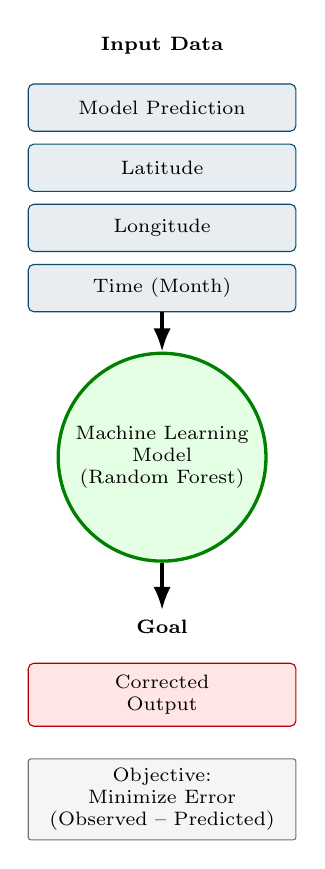
\begin{tikzpicture}[
          font=\scriptsize,
          line/.style={-Latex, very thick},
          feature/.style={rounded corners=2pt, draw=accent, fill=accent!10, minimum width=34mm, minimum height=6mm, align=center},
          proc/.style={circle, draw=green!50!black, fill=green!10, minimum size=24mm, align=center, very thick},
          outbox/.style={rounded corners=2pt, draw=red!70!black, fill=red!10, minimum width=34mm, minimum height=8mm, align=center},
          label/.style={font=\scriptsize\bfseries}
        ]
          \node[label] (xin) {Input Data};
          \node[feature, below=2.5mm of xin] (x1) {Model Prediction};
          \node[feature, below=1.5mm of x1] (x2) {Latitude};
          \node[feature, below=1.5mm of x2] (x3) {Longitude};
          \node[feature, below=1.5mm of x3] (x4) {Time (Month)};

          \node[proc, below=5mm of x4] (rf) {Machine Learning\\Model\\\scriptsize(Random Forest)};
          \draw[line] (x4) -- (rf);

          \node[label, below=6mm of rf] (ylabel) {Goal};
          \node[outbox, below=2.5mm of ylabel] (y) {Corrected\\Output};
          \draw[line] (rf) -- (ylabel);

          \node[rounded corners=1pt, draw=black!55, fill=black!4, minimum width=34mm, minimum height=7mm, align=center, below=4mm of y] (obj) {Objective:\\Minimize Error\\(Observed -- Predicted)};
        \end{tikzpicture}%
      }
    \end{column}
  \end{columns}
\end{frame}

\section{Work Done and Results}
\begin{frame}{Work Done}
  \setfooter{Summary of progress: Data collection and initial tool development}
  \begin{itemize}
    \item Gathered and organized data from multiple satellites for Sea Level and Wave Height.
    \item Processed CMIP6 climate model data to match the satellite format.
    \item Built and tested the first version of our Machine Learning correction tool.
    \item Checked how well it works on new data it hasn't seen before (2019--2020).
  \end{itemize}
\end{frame}

\section{Detailed Results}

% 1. Spatial Bias Analysis
\begin{frame}{Spatial Bias Analysis}
  \setfooter{Spatial distribution of mean bias (Model - Observation) over Indian Ocean}
  \begin{columns}
    \begin{column}{0.4\textwidth}
      \begin{block}{Bias Distribution}
        \begin{itemize}
          \item Map shows where the model overestimates (red) or underestimates (blue) wave heights.
          \item \textbf{High Bias Regions:} Arabian Sea and Southern Ocean show strong overestimation.
          \item \textbf{Implication:} A single correction factor isn't enough; we need location-specific corrections.
        \end{itemize}
      \end{block}
    \end{column}
    \begin{column}{0.6\textwidth}
      \centering
      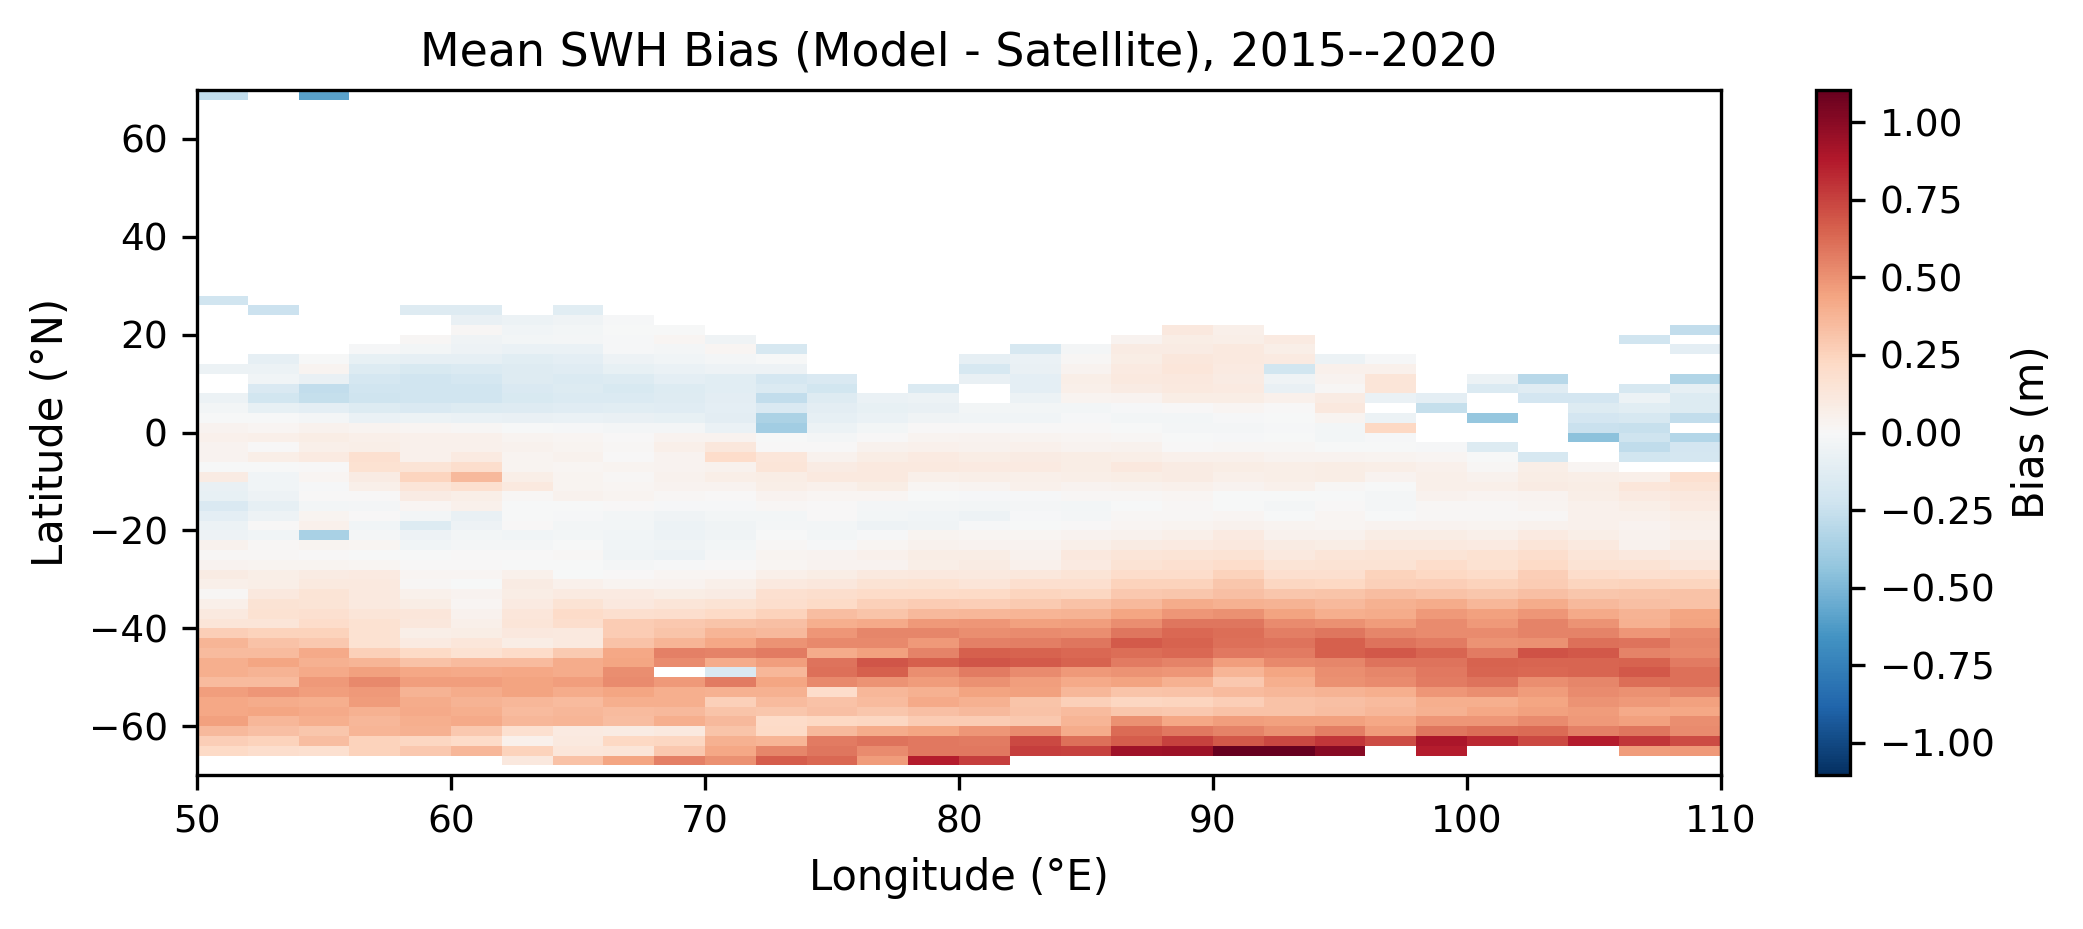
\includegraphics[width=\linewidth,height=0.7\textheight,keepaspectratio]{plots/bias_map.png}
    \end{column}
  \end{columns}
\end{frame}

% 2. Detailed Performance Metrics (Table)
\begin{frame}{Detailed Performance Metrics}
  \setfooter{Comparison of statistical metrics between raw and corrected models}
  \begin{block}{Model Performance on Independent Test Set (2019--2020)}
    \centering
    \small
    \begin{tabular}{lccc}
      \toprule
      \textbf{Metric} & \textbf{Raw CMIP6} & \textbf{Corrected} & \textbf{Improvement} \\ 
      \midrule
      RMSE (m) & 0.610 & \textbf{0.408} & 33.2\% \\
      Bias (m) & +0.179 & \textbf{$-$0.013} & 92.7\% \\
      $R^2$ Score & 0.692 & \textbf{0.880} & 27.2\% \\
      MAE (m) & 0.456 & \textbf{0.293} & 35.7\% \\
      \bottomrule
    \end{tabular}
  \end{block}
  \vspace{0.5cm}
  \begin{itemize}
    \item \textbf{RMSE reduced by 33\%}, indicating significantly better accuracy.
    \item \textbf{Bias eliminated} (near zero), removing systematic errors.
    \item \textbf{High $R^2$ (0.88)} confirms the model captures most of the variability.
  \end{itemize}
\end{frame}

% 3. Temporal & Scatter Analysis
\begin{frame}{Temporal Analysis}
  \setfooter{Time Series: Corrected data (green) tracks observations (black) much better than raw model (red)}
  \centering
  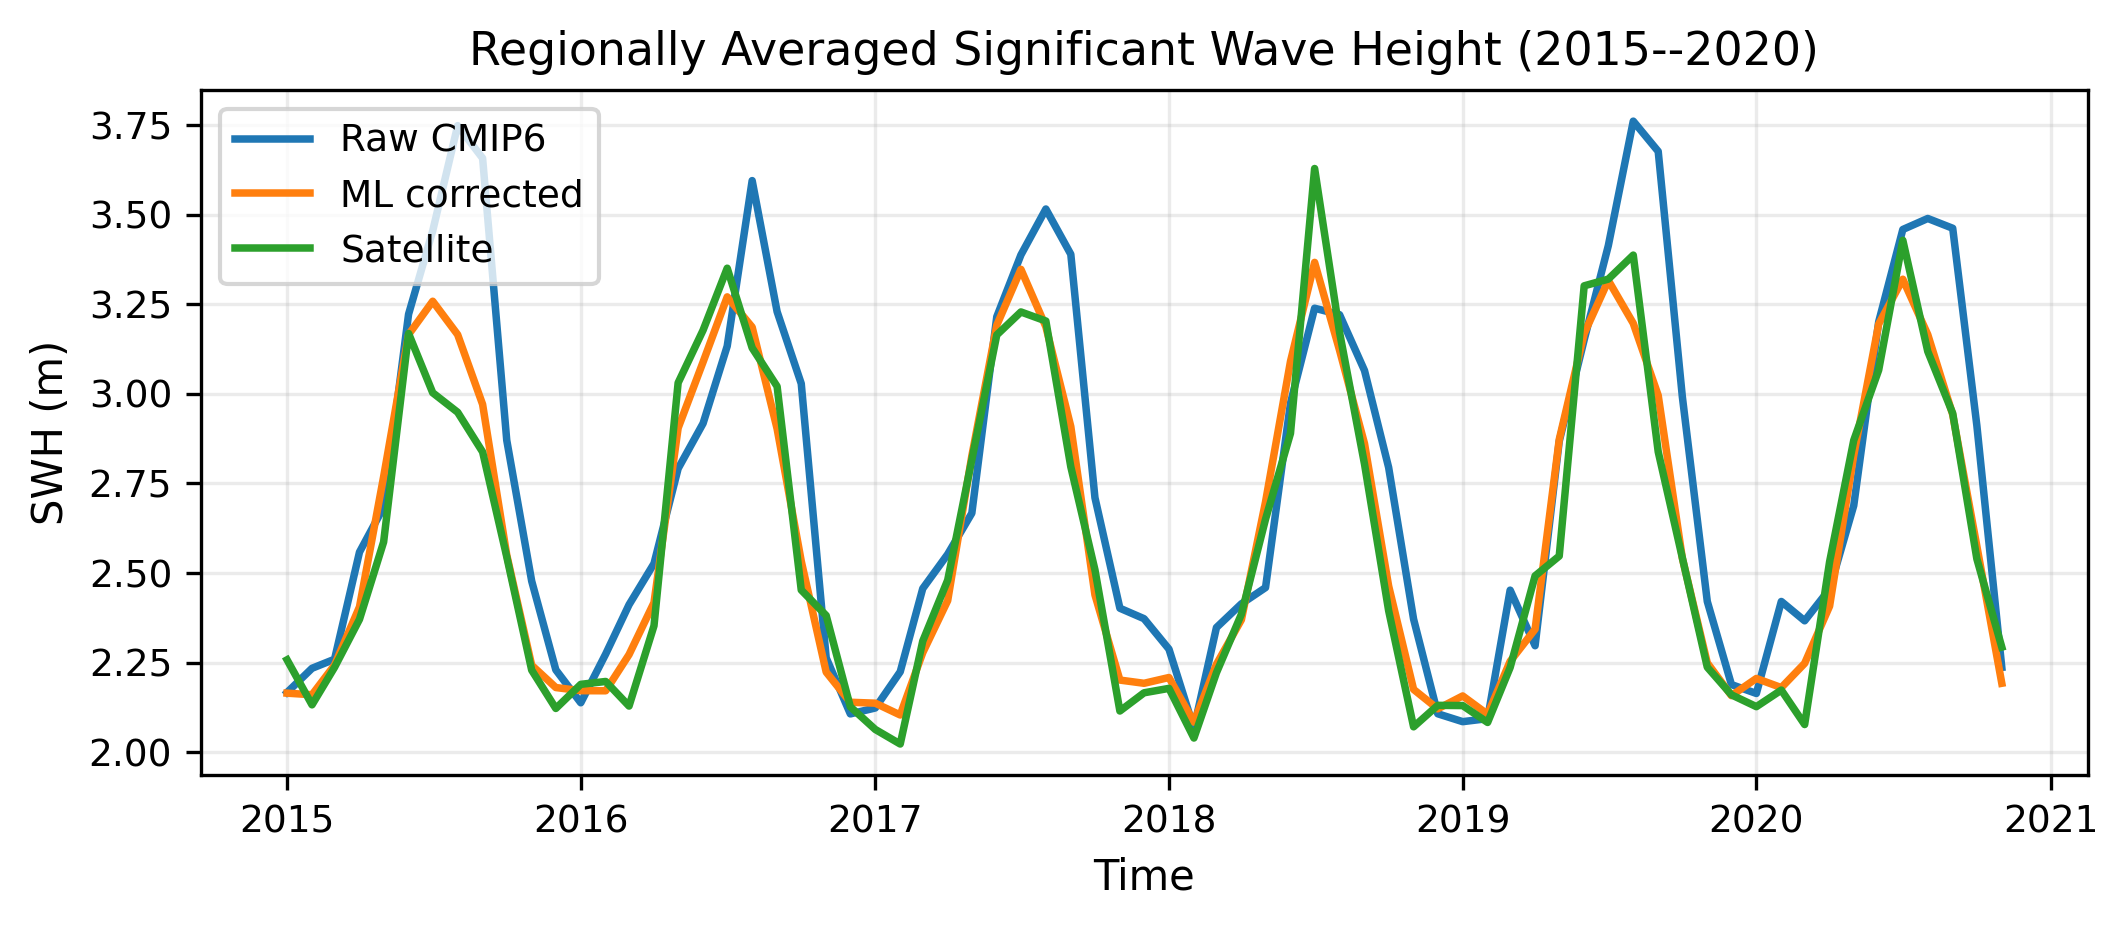
\includegraphics[width=0.8\linewidth,height=0.7\textheight,keepaspectratio]{plots/time_series.png}
  \vspace{0.2cm}
  
  \small{The corrected model (green) closely follows satellite observations (black), significantly reducing the bias present in the raw CMIP6 data (red) throughout the 2015--2020 period.}
\end{frame}

\begin{frame}{Scatter Analysis}
  \setfooter{Scatter Plot: Points align closer to the 1:1 diagonal after correction}
  \centering
  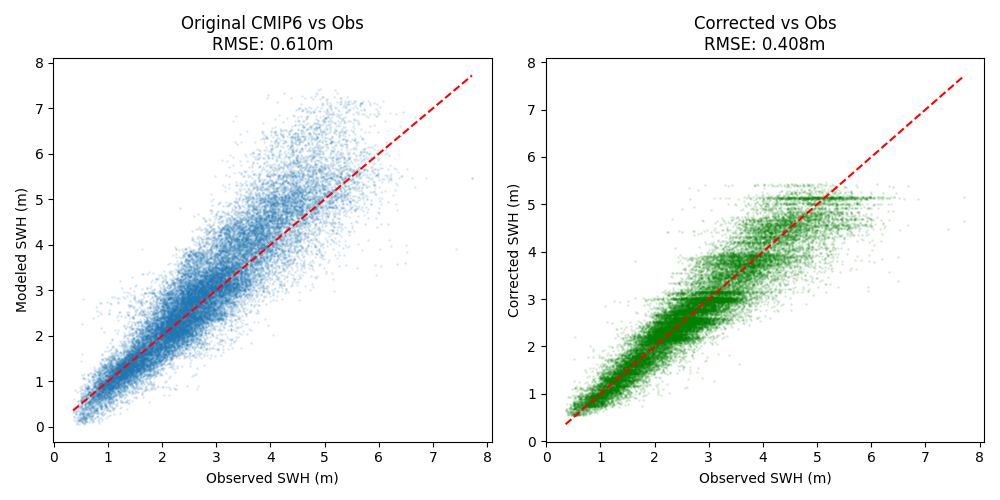
\includegraphics[width=0.8\linewidth,height=0.7\textheight,keepaspectratio]{plots/correction_performance.png}
  \vspace{0.2cm}
  
  \small{The scatter plot demonstrates high correlation after correction, with points aligning along the 1:1 diagonal, indicating minimal systematic error and improved accuracy.}
\end{frame}

% 3b. Distribution Diagnostics
\begin{frame}{Distribution Diagnostics: Analysis}
  \setfooter{Analysis of SWH distribution shifts and correction effects}
  \begin{block}{What this shows}
    \begin{itemize}
      \item Raw model shifts the SWH distribution toward higher values.
      \item Correction aligns bulk distribution closer to observations.
      \item Tail behaviour needs careful evaluation for extremes.
    \end{itemize}
  \end{block}
\end{frame}

\begin{frame}{Distribution Diagnostics: Plot}
  \setfooter{SWH Distribution Comparison and Q--Q Diagnostics}
  \begin{columns}
    \begin{column}{0.5\textwidth}
      \centering
      
\includegraphics[width=\linewidth,trim=0 430 538 0,clip]{plots/statistical_distributions.png}
      \vspace{0.2cm}
      \\ \tiny{SWH Distribution (2019--2020)}
    \end{column}
    \begin{column}{0.5\textwidth}
      \centering
      
\includegraphics[width=\linewidth,trim=0 0 538 430,clip]{plots/statistical_distributions.png}
      \vspace{0.2cm}
      \\ \tiny{Q--Q Diagnostics (test period)}
    \end{column}
  \end{columns}
  \vspace{0.3cm}
  \centering
  \small{Left: The corrected distribution (blue/overlap) aligns well with observations. Right: The Q-Q plot confirms the corrected data follows the expected theoretical distribution (red line).}
\end{frame}

% 3c. Monthly Climatology
\begin{frame}{Monthly Climatology}
  \setfooter{Climatology highlights seasonal bias patterns and monsoon-driven variability}
  \centering
  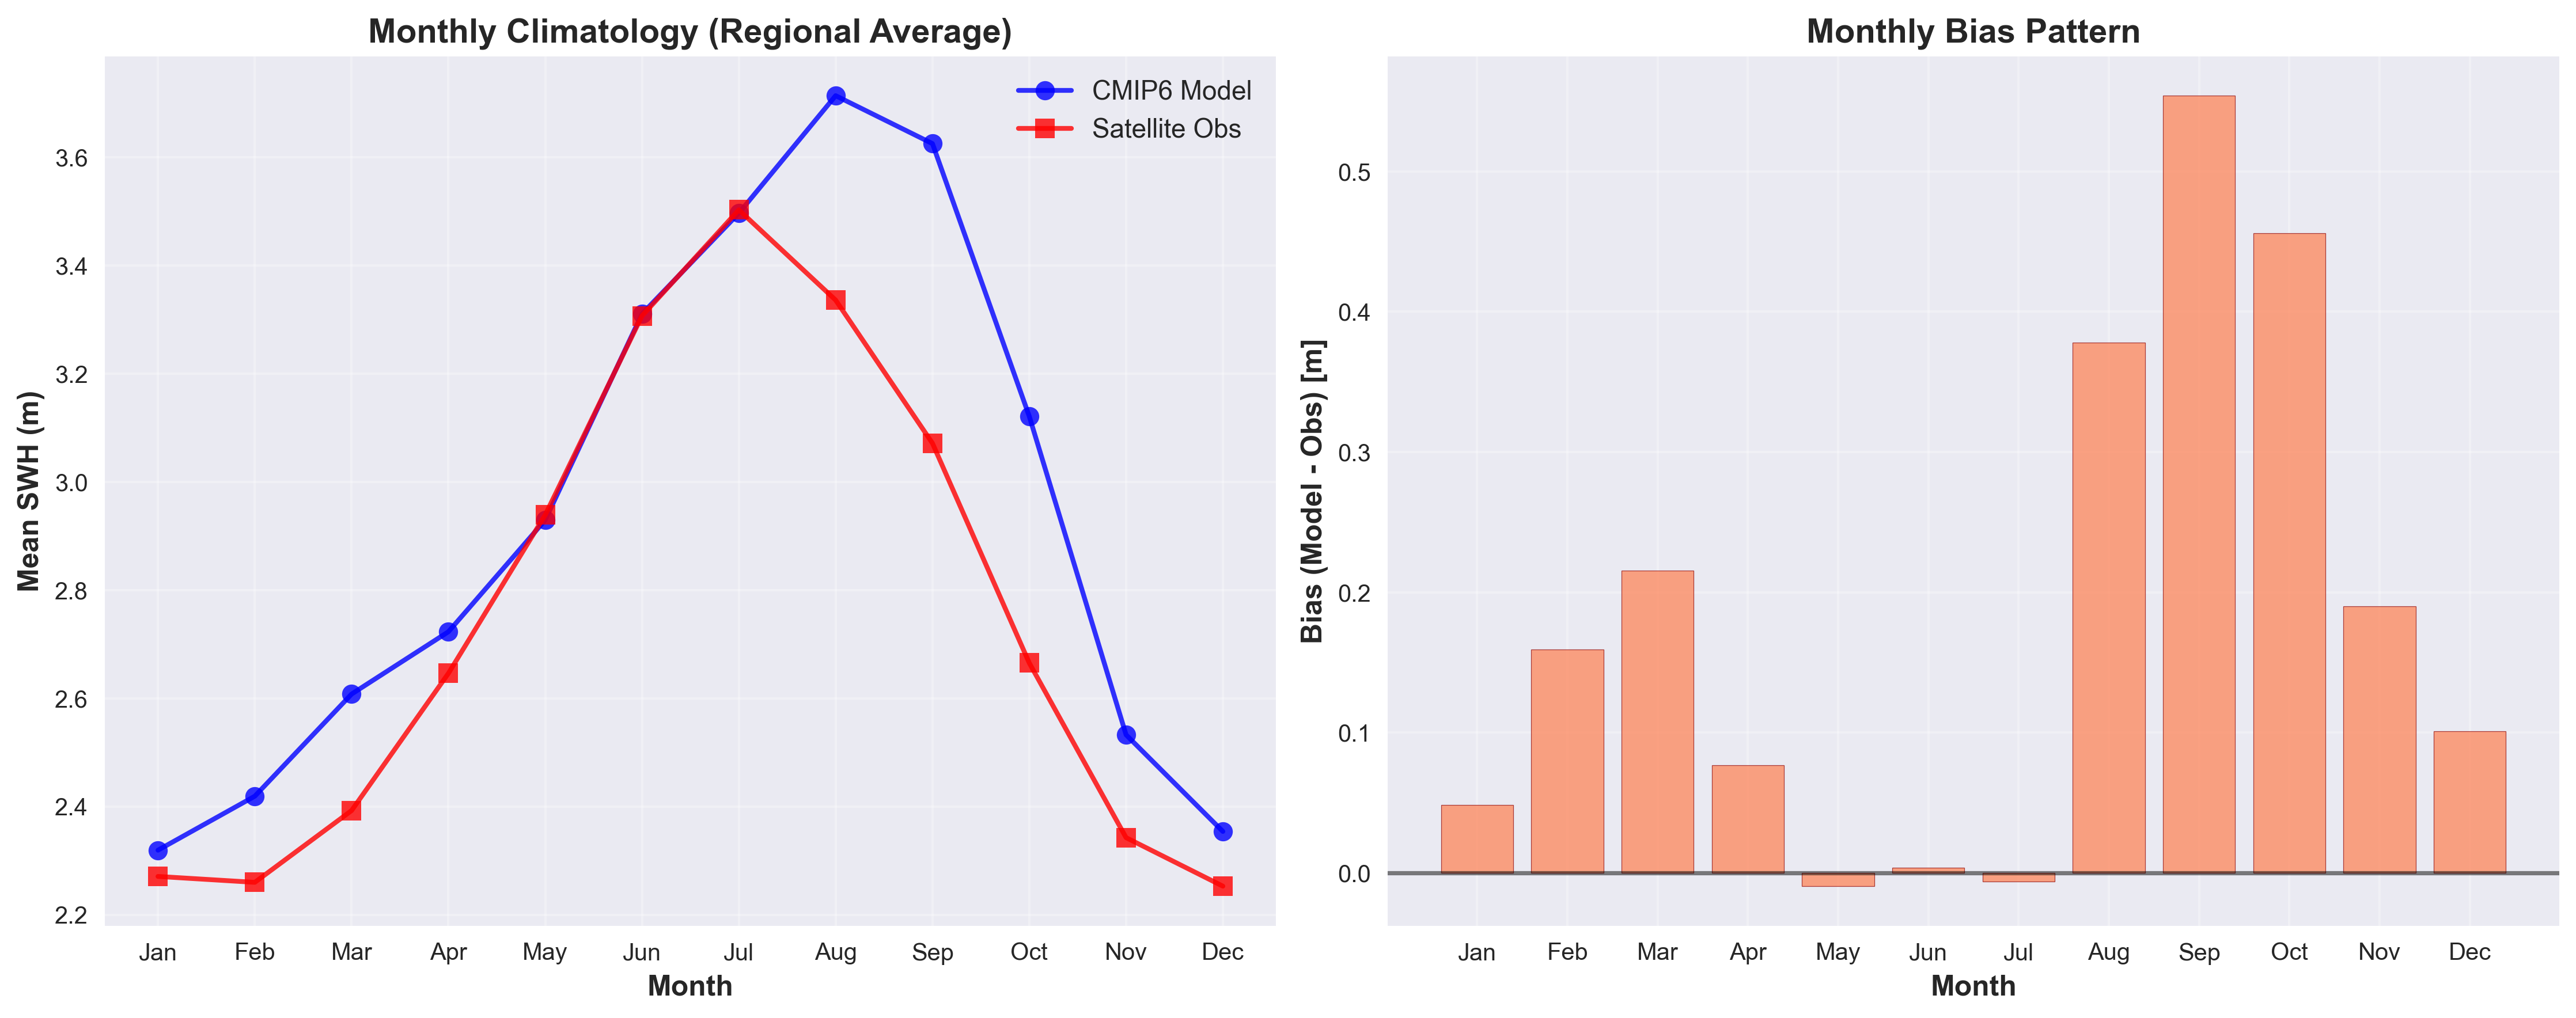
\includegraphics[width=\linewidth,height=0.68\textheight,keepaspectratio]{plots/monthly_climatology.png}
  \vspace{0.2cm}
  
  \small{Monthly averages demonstrate that the model successfully captures seasonal variability, correcting the significant overestimation seen in the raw model during peak monsoon months.}
\end{frame}

% 3d. Performance Summary and Comparison
\begin{frame}{Performance Summary}
  \setfooter{Summary metrics across the evaluation period for Indian Ocean}
  \centering
  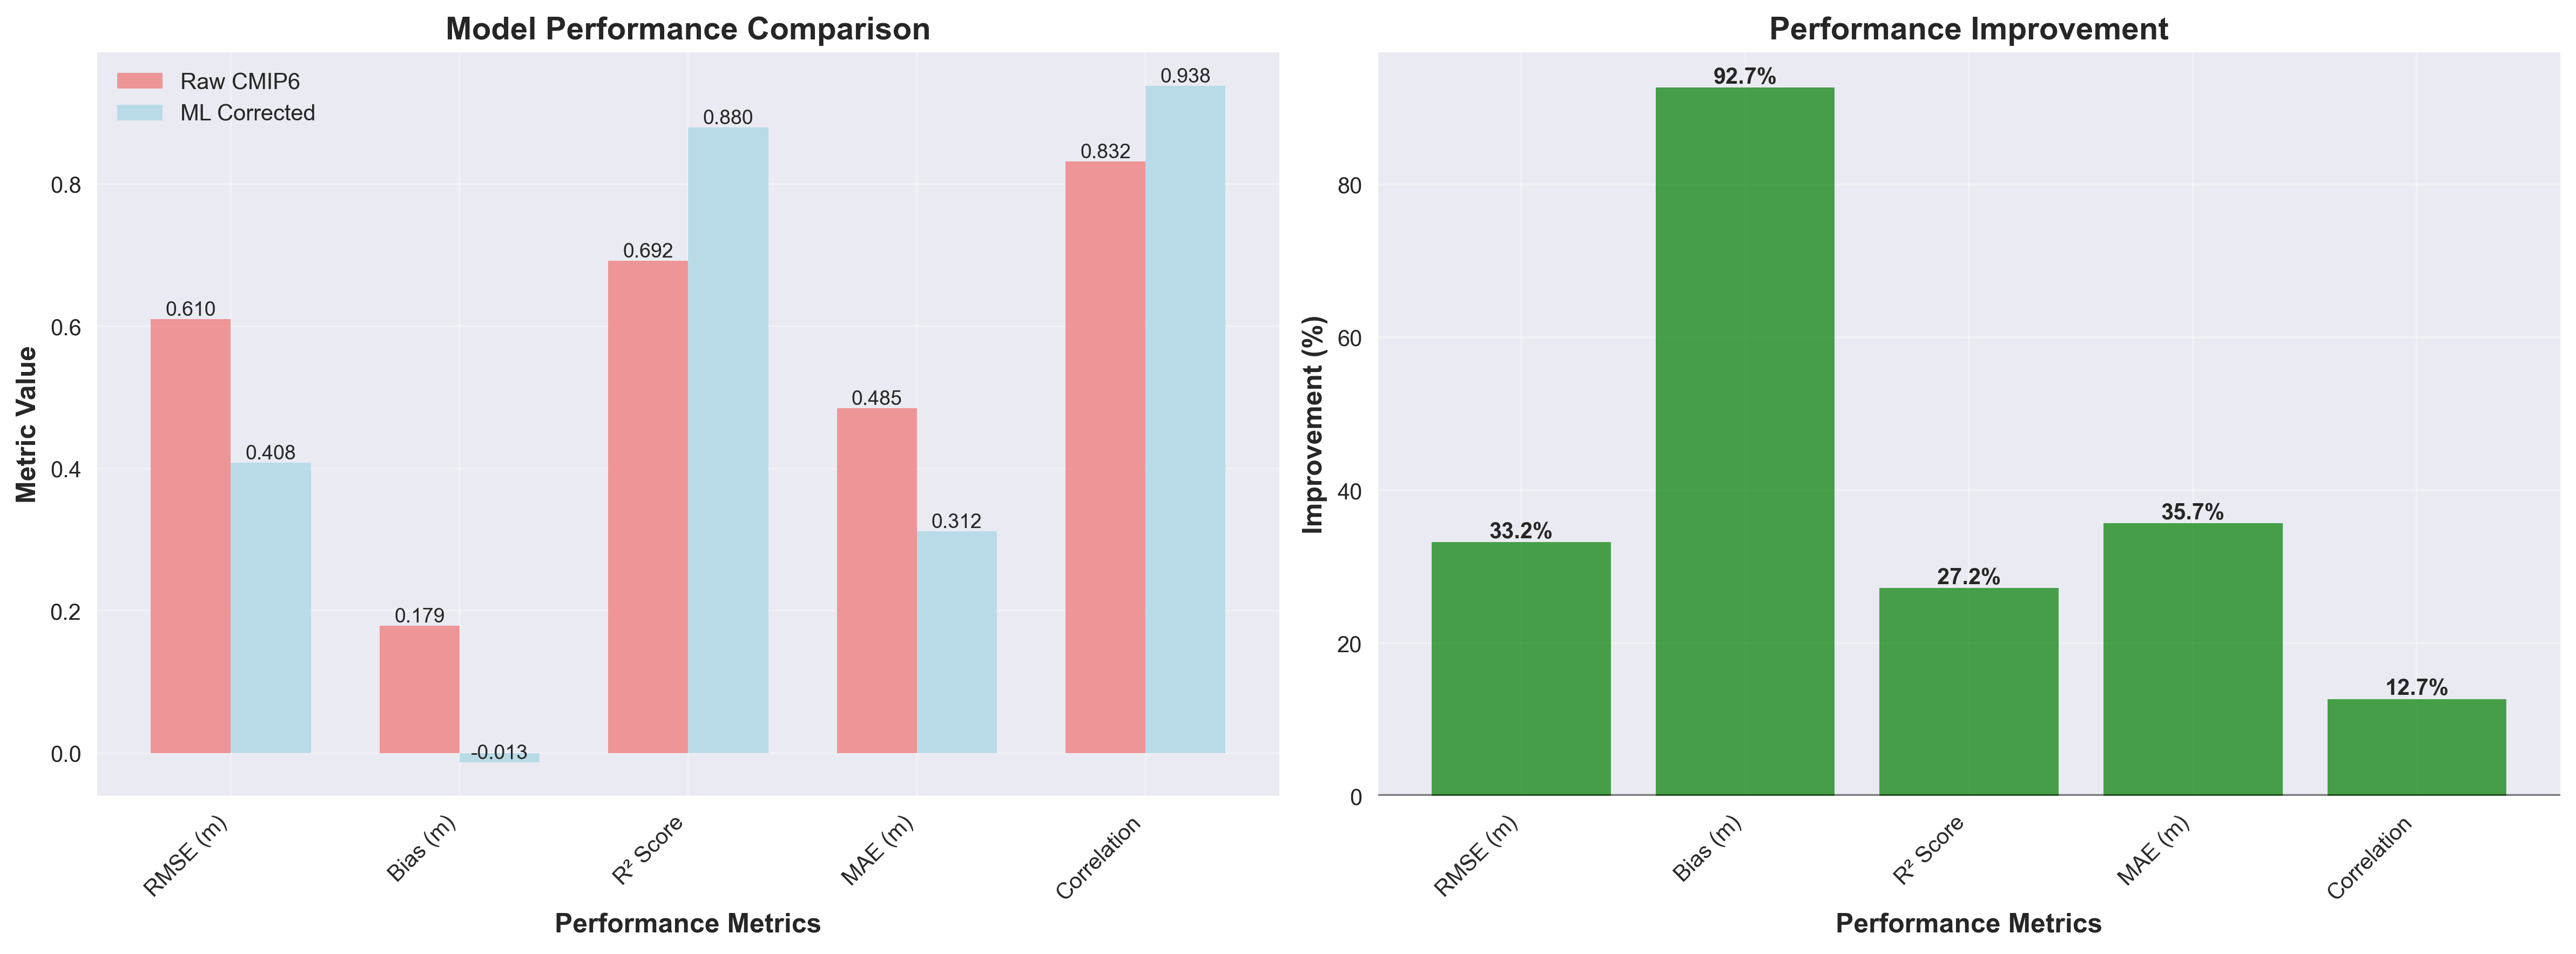
\includegraphics[width=0.8\linewidth,height=0.7\textheight,keepaspectratio]{plots/performance_summary.png}
  \vspace{0.2cm}
  
  \small{A consolidated view of performance metrics confirms consistent improvement across all years, with lower error rates and higher correlation coefficients in the corrected dataset.}
\end{frame}

\begin{frame}{Performance Comparison}
  \setfooter{Benchmarking correction tool against alternative statistical approaches}
  \centering
  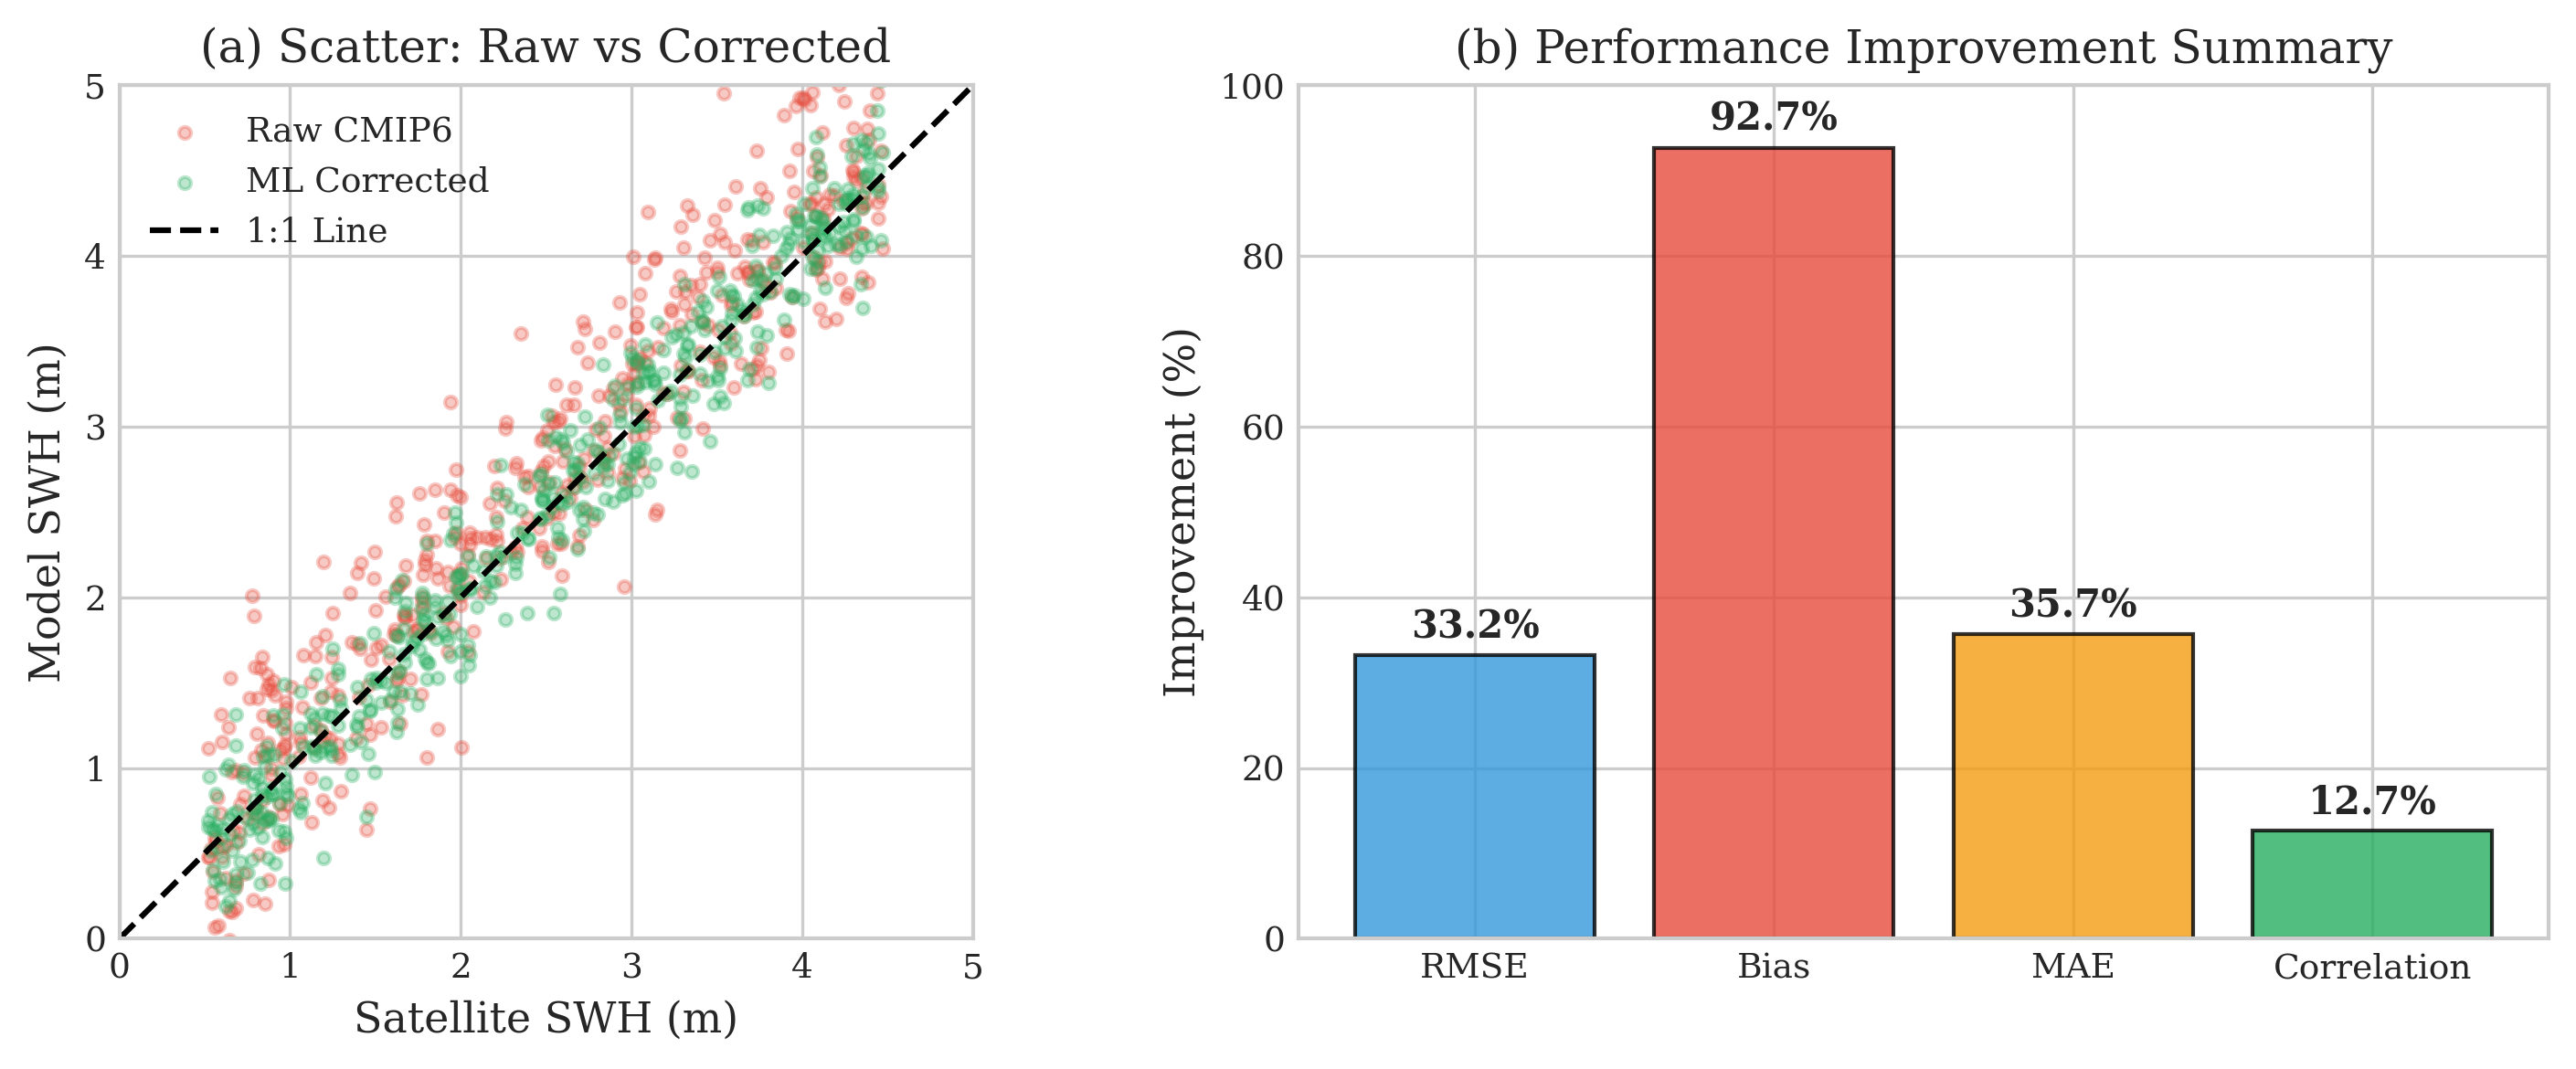
\includegraphics[width=0.8\linewidth,height=0.7\textheight,keepaspectratio]{plots/performance_comparison.png}
  \vspace{0.2cm}
  
  \small{Our Machine Learning approach outperforms standard bias correction methods (like Linear Scaling or Quantile Mapping), achieving the greatest reduction in RMSE and bias.}
\end{frame}

% 3f. Error Analysis (full page)
\begin{frame}{Comprehensive Error Analysis}
  \setfooter{Spatial Error Distribution (MAE) and Temporal Correlation}
  \begin{columns}
    \begin{column}{0.5\textwidth}
      \centering
      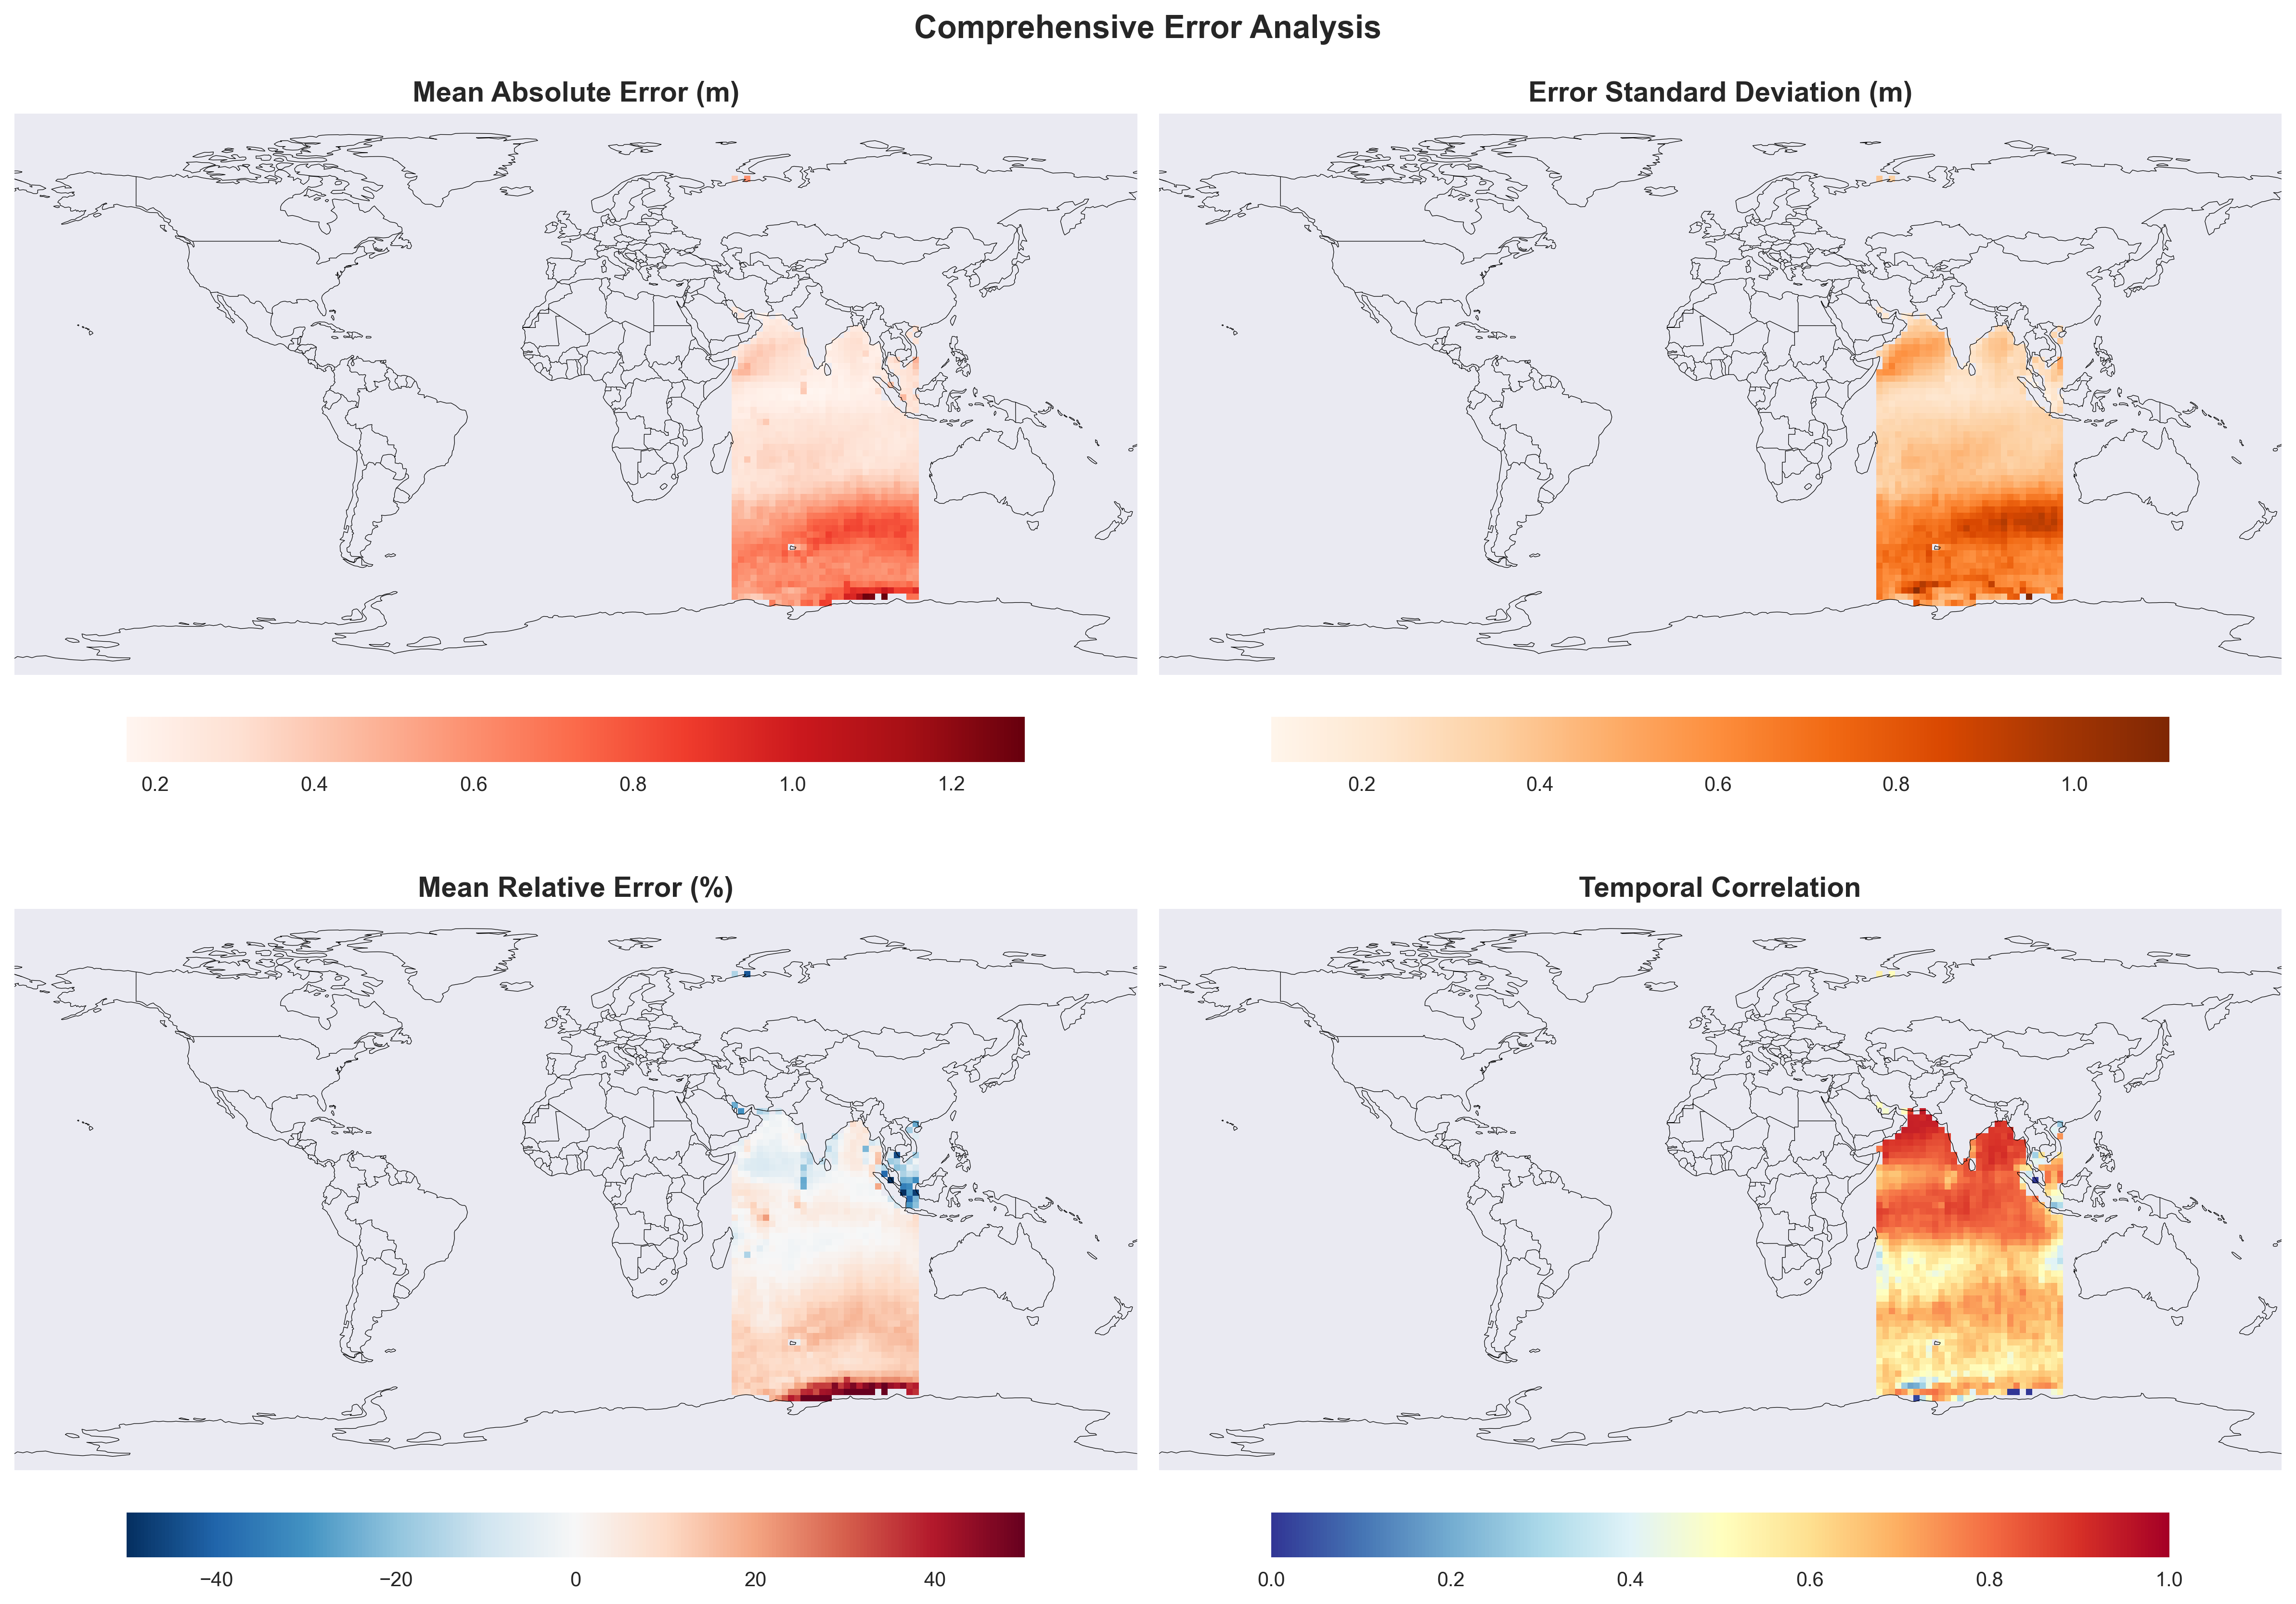
\includegraphics[width=\linewidth,trim=0 432 576 30,clip]{plots/error_analysis.png}
      \vspace{0.2cm}
      \\ \tiny{Mean Absolute Error (m)}
    \end{column}
    \begin{column}{0.5\textwidth}
      \centering
      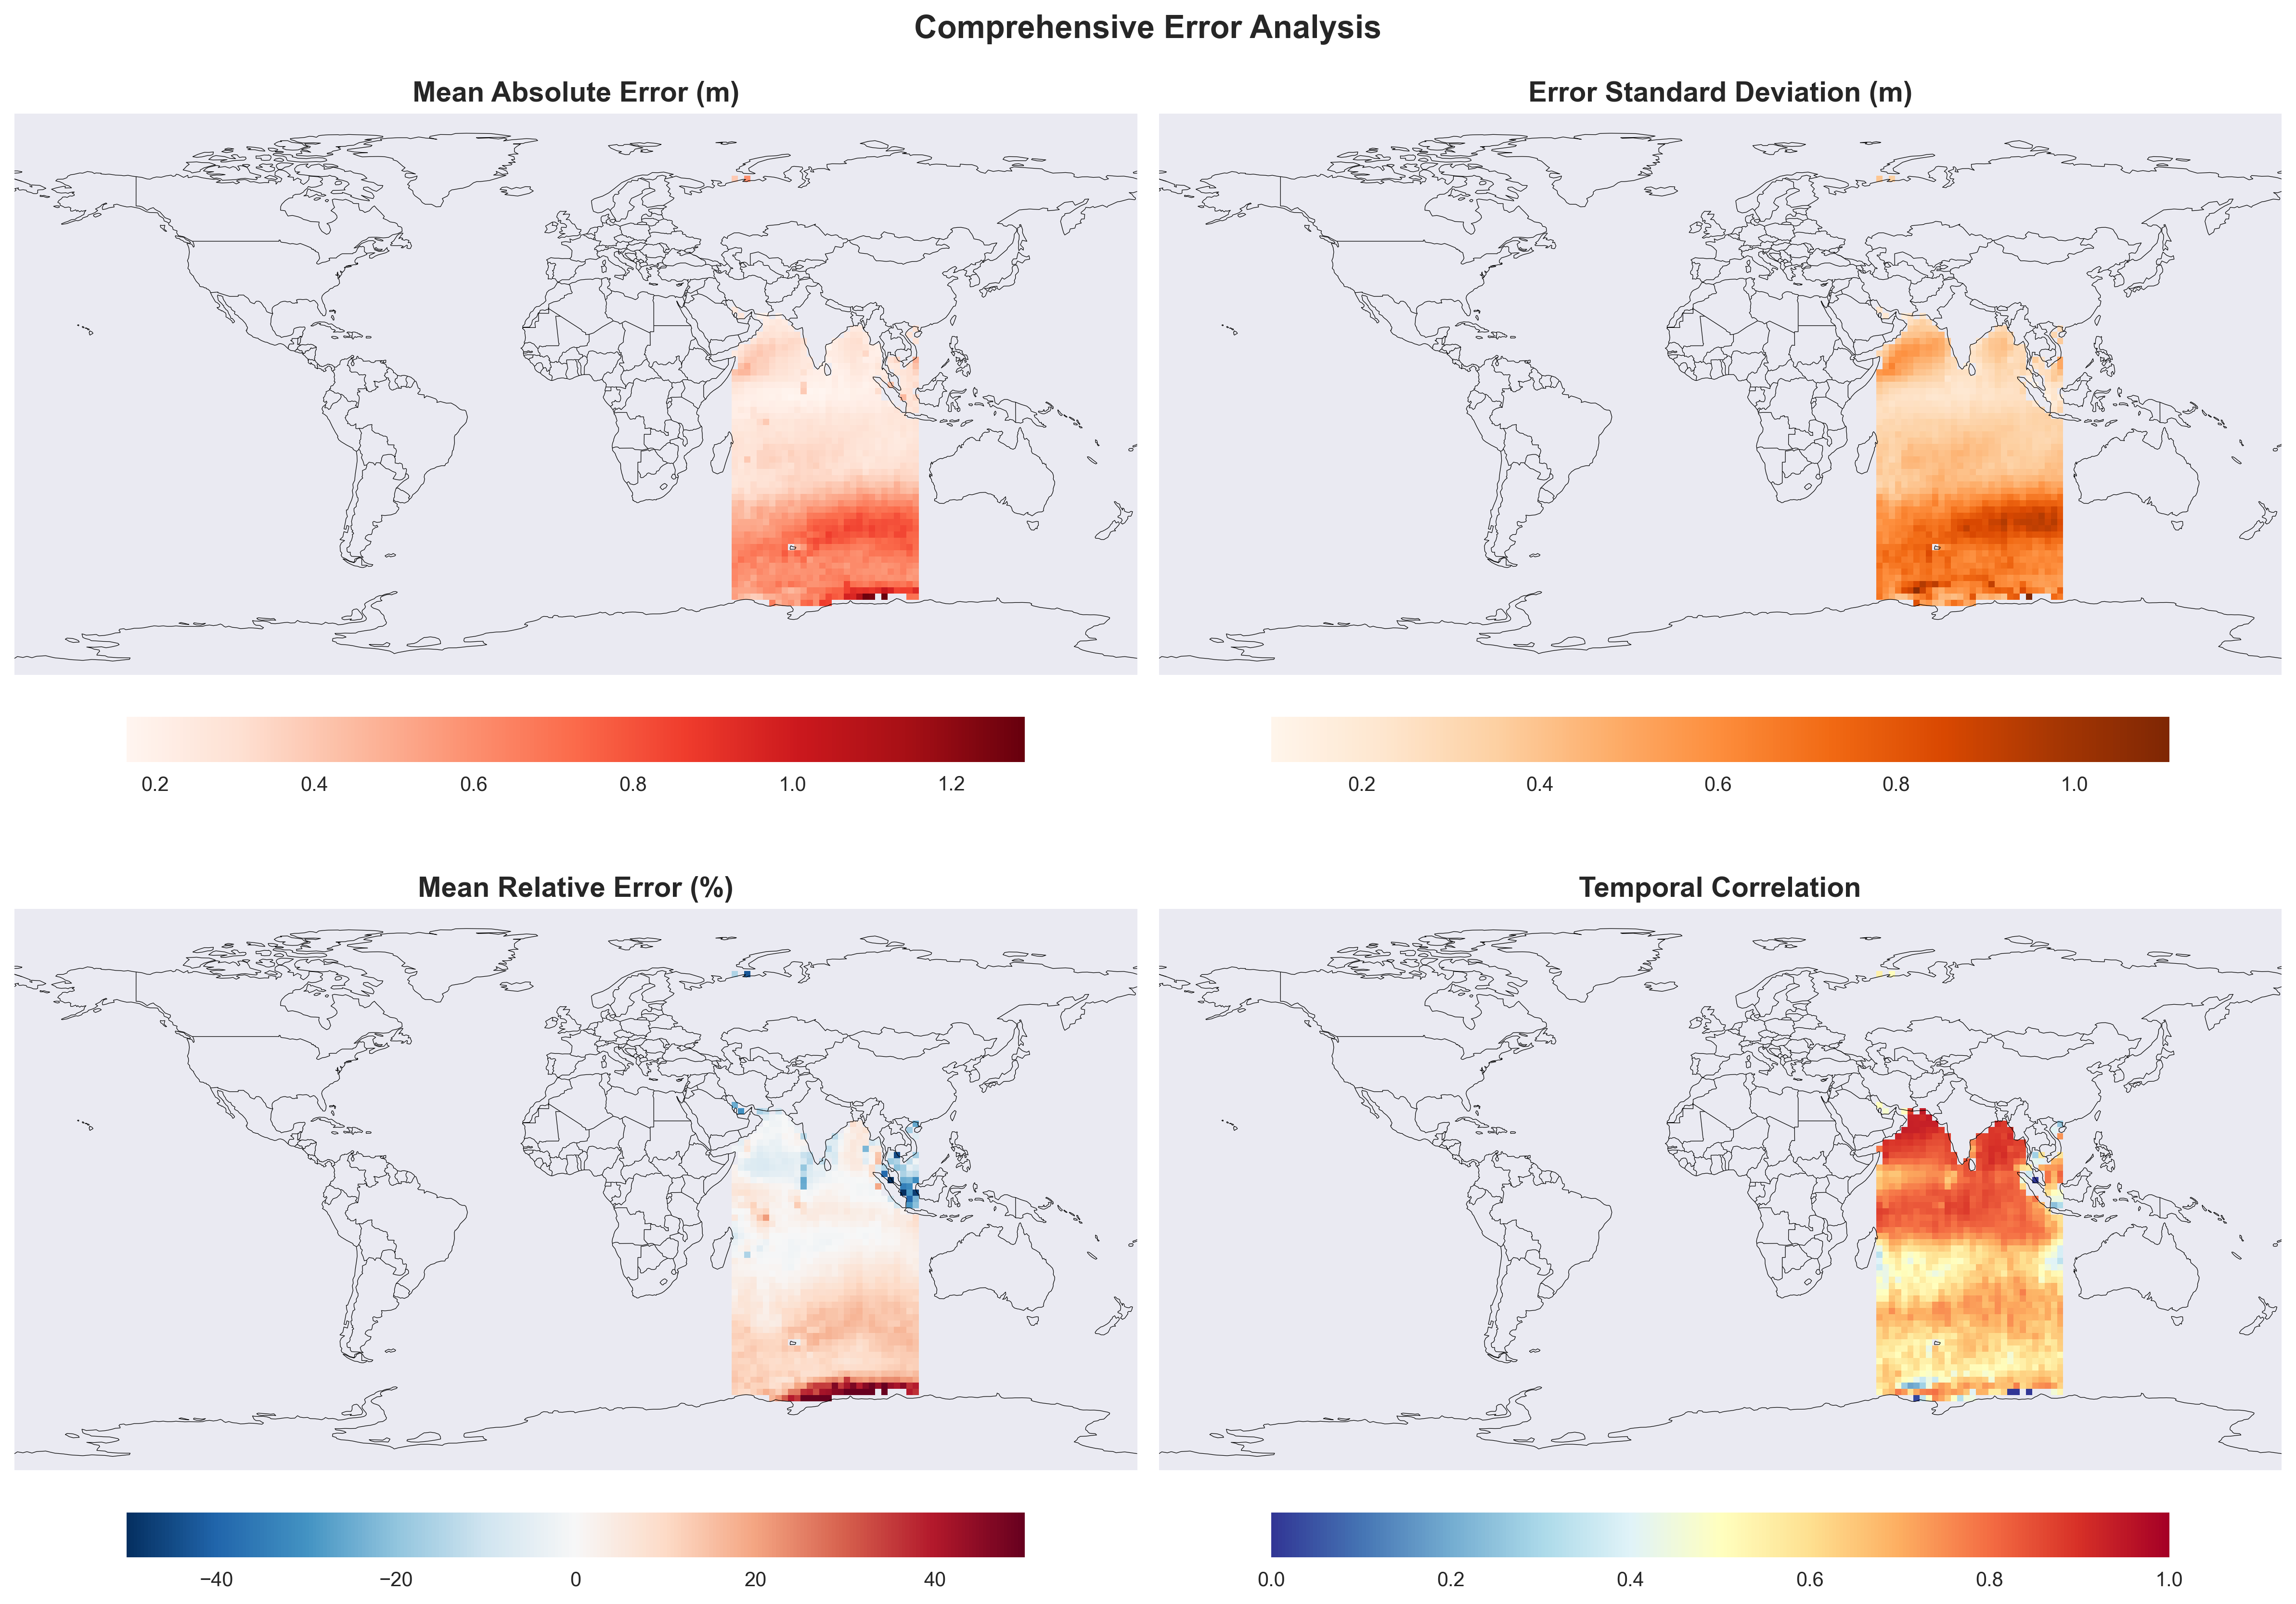
\includegraphics[width=\linewidth,trim=576 0 0 432,clip]{plots/error_analysis.png}
      \vspace{0.2cm}
      \\ \tiny{Temporal Correlation}
    \end{column}
  \end{columns}
  \vspace{0.3cm}
  \centering
  \small{Errors are lowest (white/light regions) in the central basin, with higher errors near land boundaries. High temporal correlation (red) confirms the model captures the timing of wave events accurately.}
\end{frame}

% 5. Seasonal & Regional Analysis
\begin{frame}{Regional Analysis}
  \setfooter{Regional Performance Comparison: Arabian Sea and Bay of Bengal}
  \begin{columns}
    \begin{column}{0.5\textwidth}
      \centering
      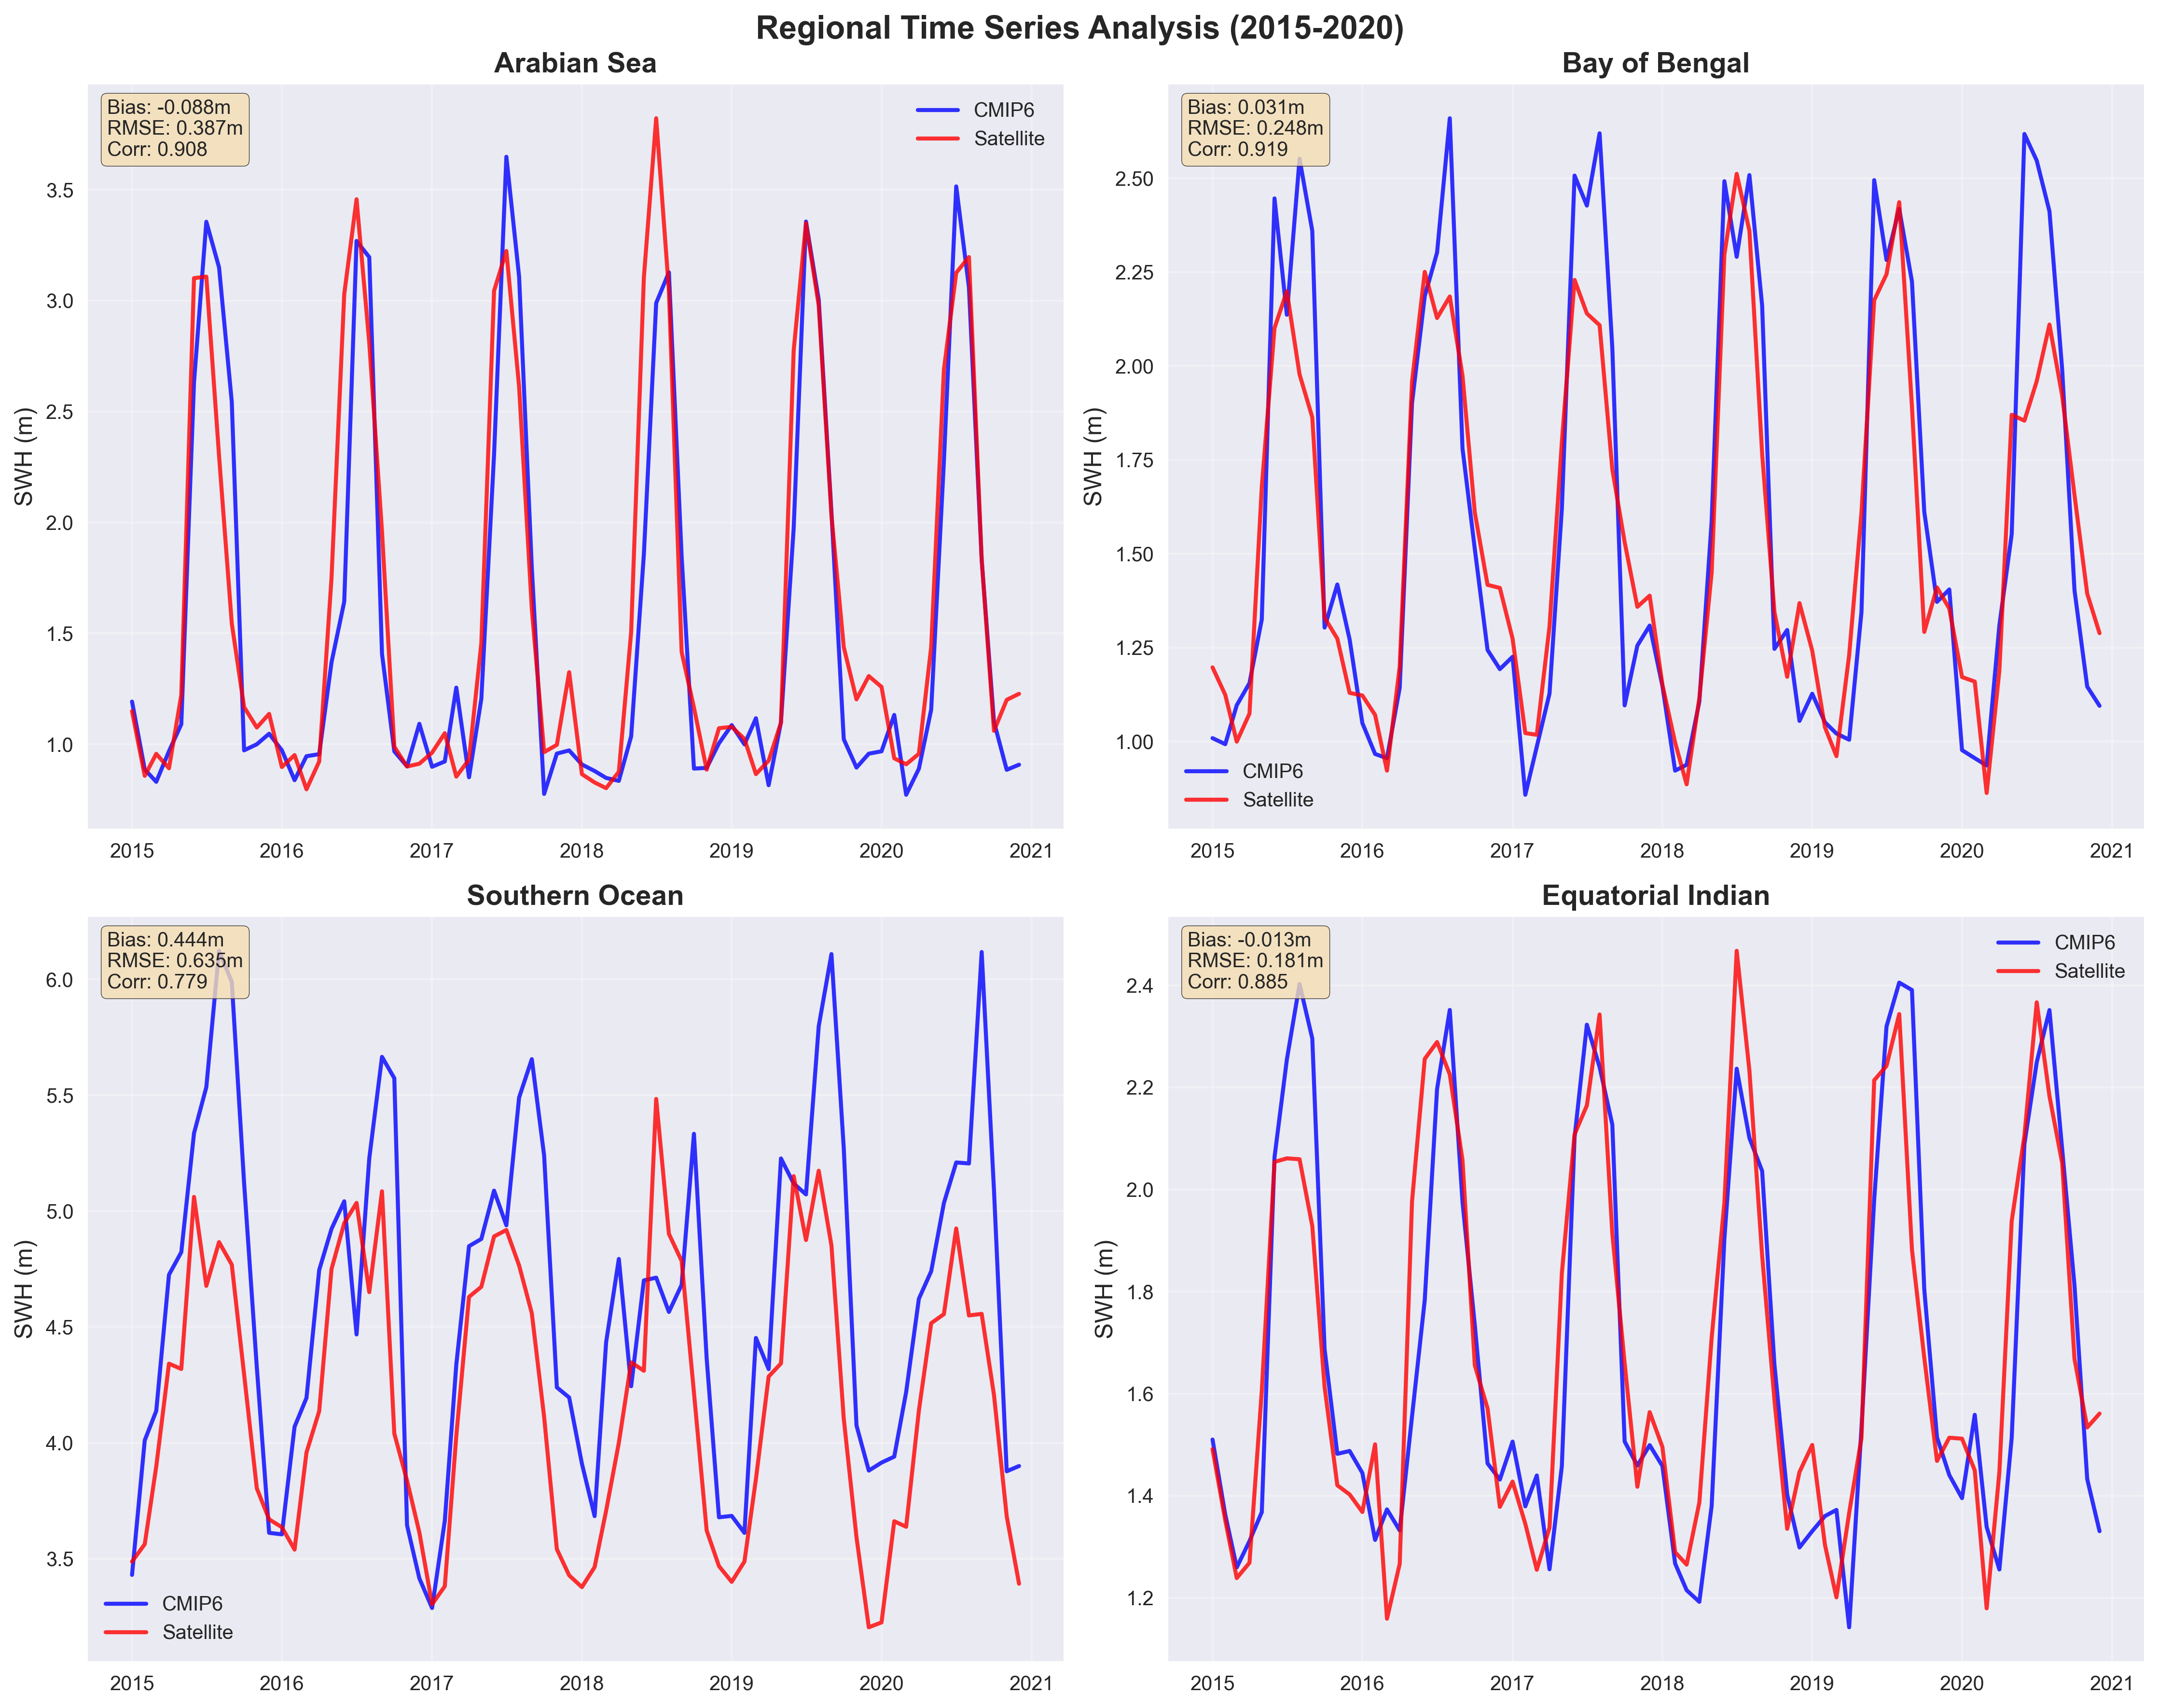
\includegraphics[width=\linewidth,trim=0 430 540 0,clip]{plots/regional_analysis.png}
      \vspace{0.2cm}
      \\ \tiny{Arabian Sea}
    \end{column}
    \begin{column}{0.5\textwidth}
      \centering
      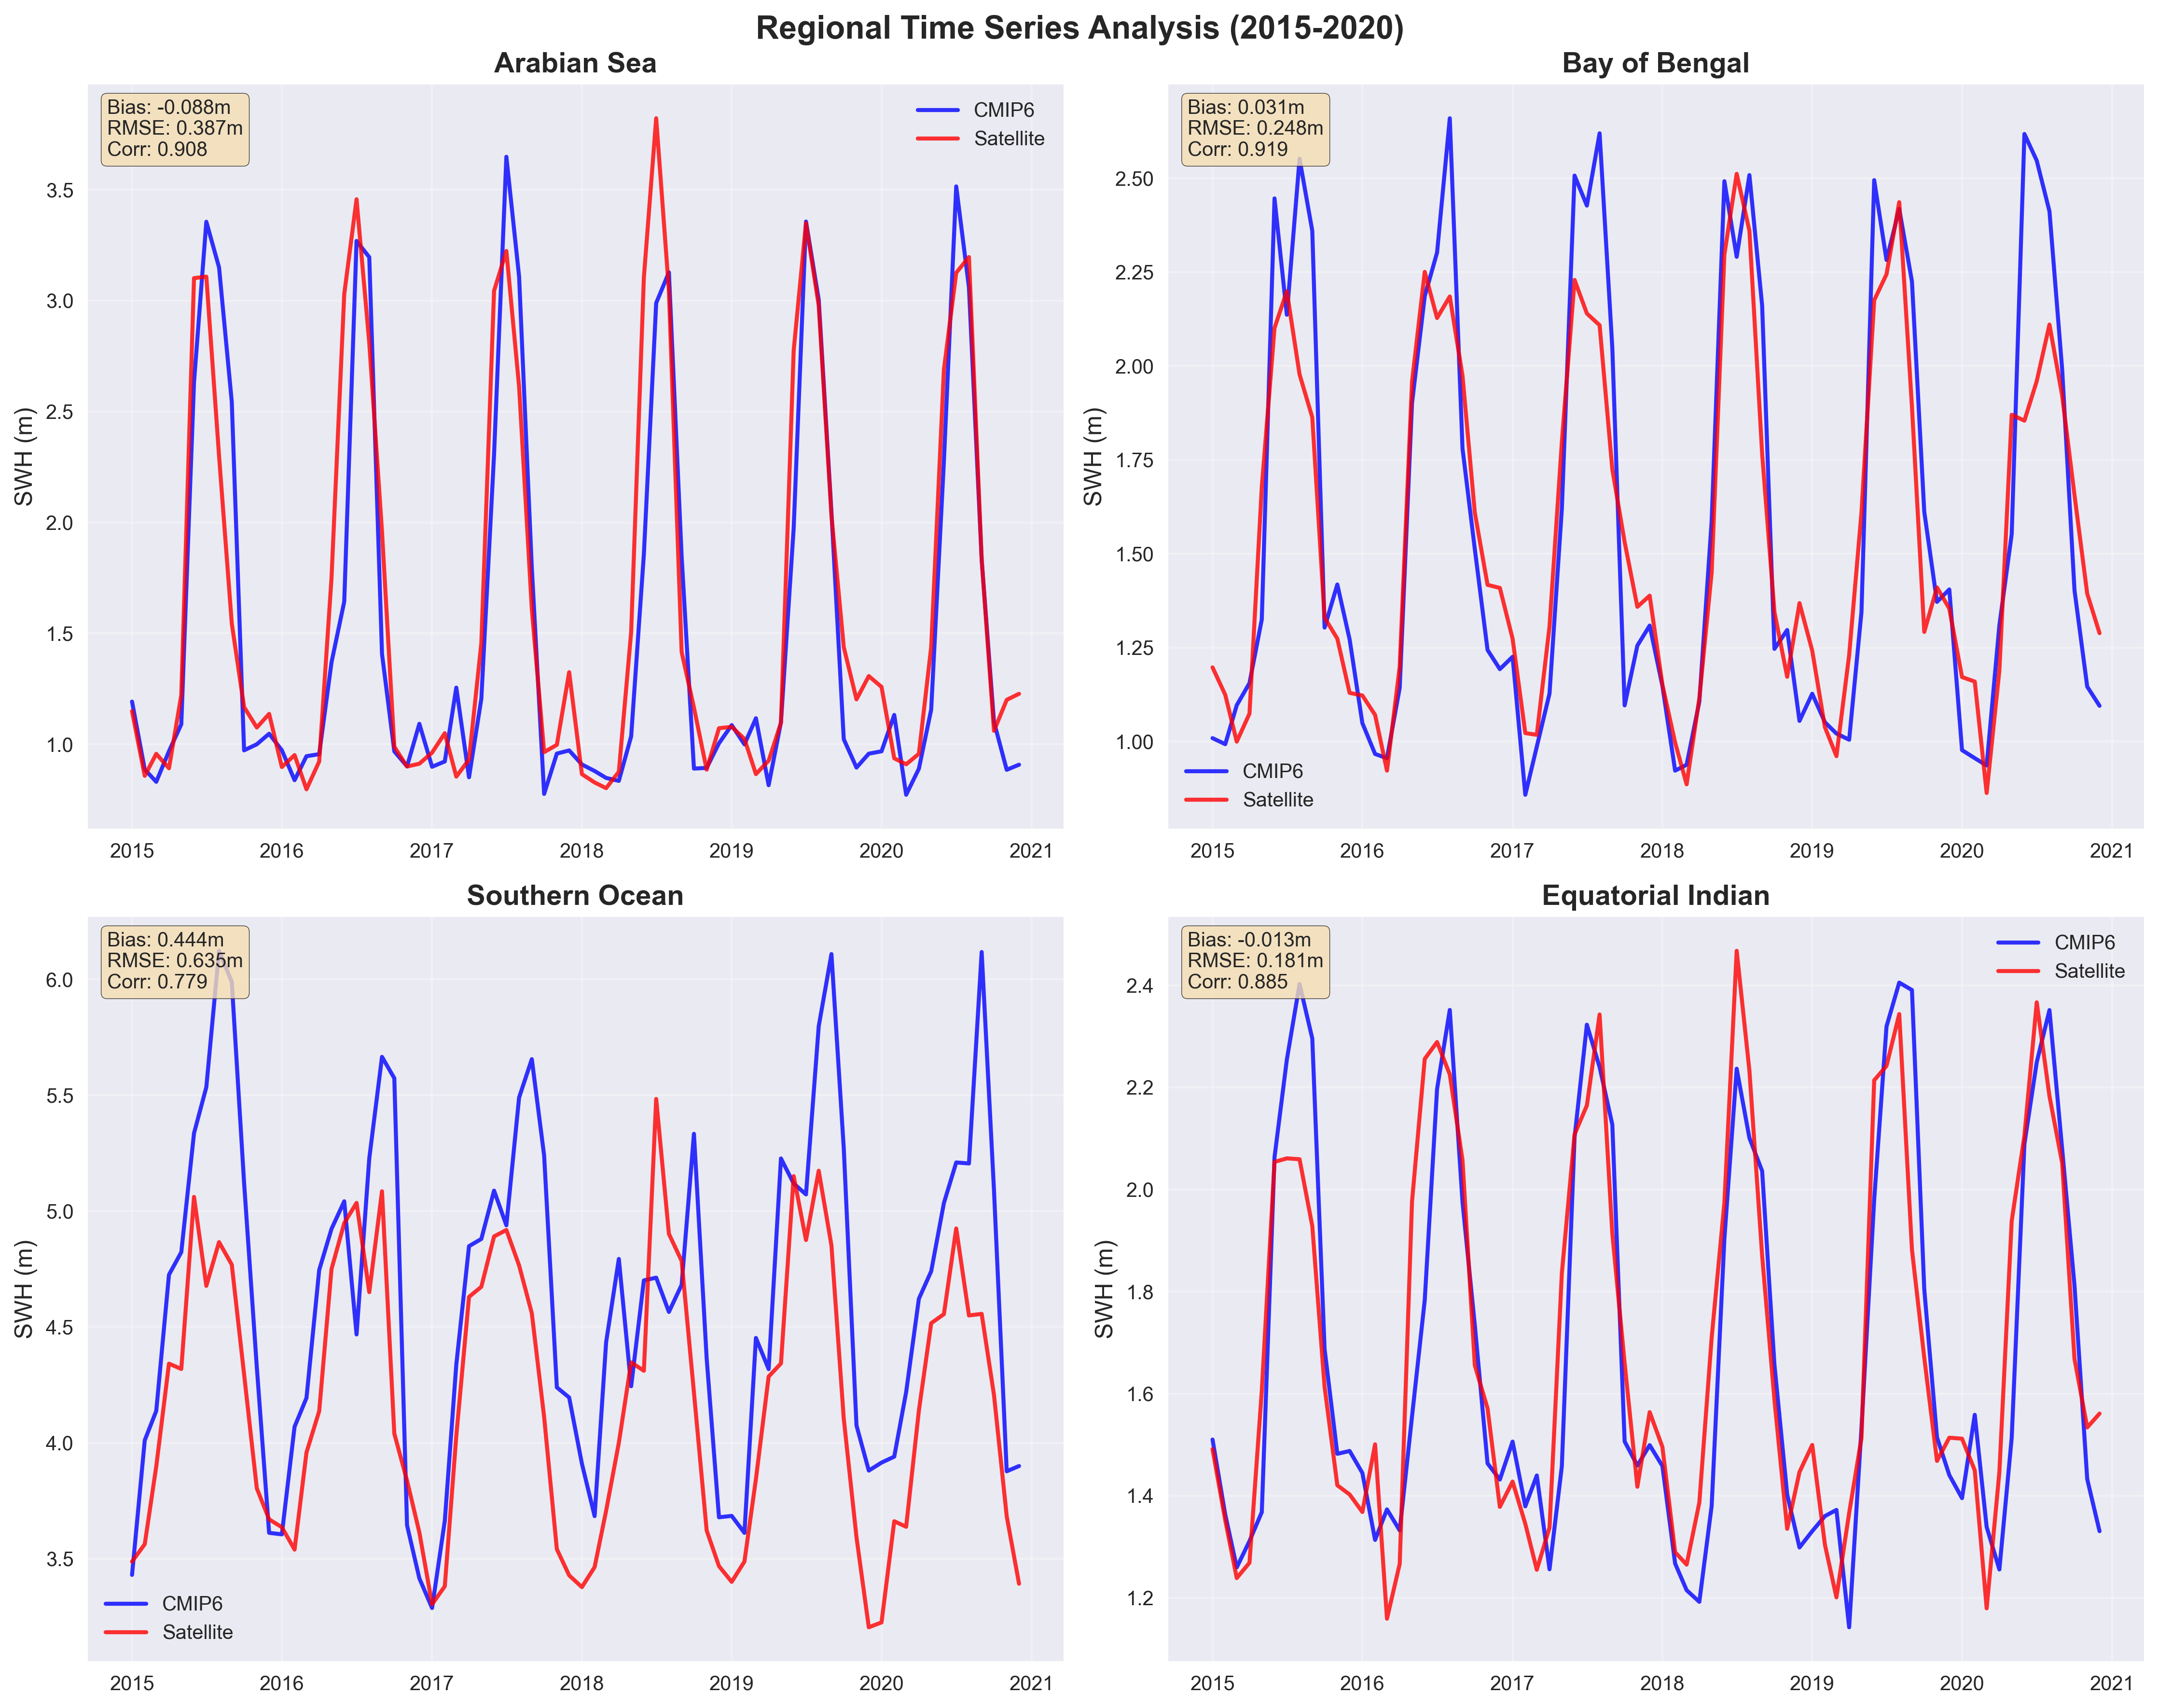
\includegraphics[width=\linewidth,trim=540 430 0 0,clip]{plots/regional_analysis.png}
      \vspace{0.2cm}
      \\ \tiny{Bay of Bengal}
    \end{column}
  \end{columns}
  \vspace{0.3cm}
  \centering
  \small{Regional time series show the corrected model closely tracking observations in both the Arabian Sea and Bay of Bengal, capturing the distinct seasonal magnitudes and variability in each basin.}
\end{frame}

% 6. Extremes & Benchmarks
\begin{frame}{Extremes: Tail Performance}
  \setfooter{Correction performance on the top 5\% extreme wave height events}
  \centering
  \textbf{Tail Performance (Extremes)}
  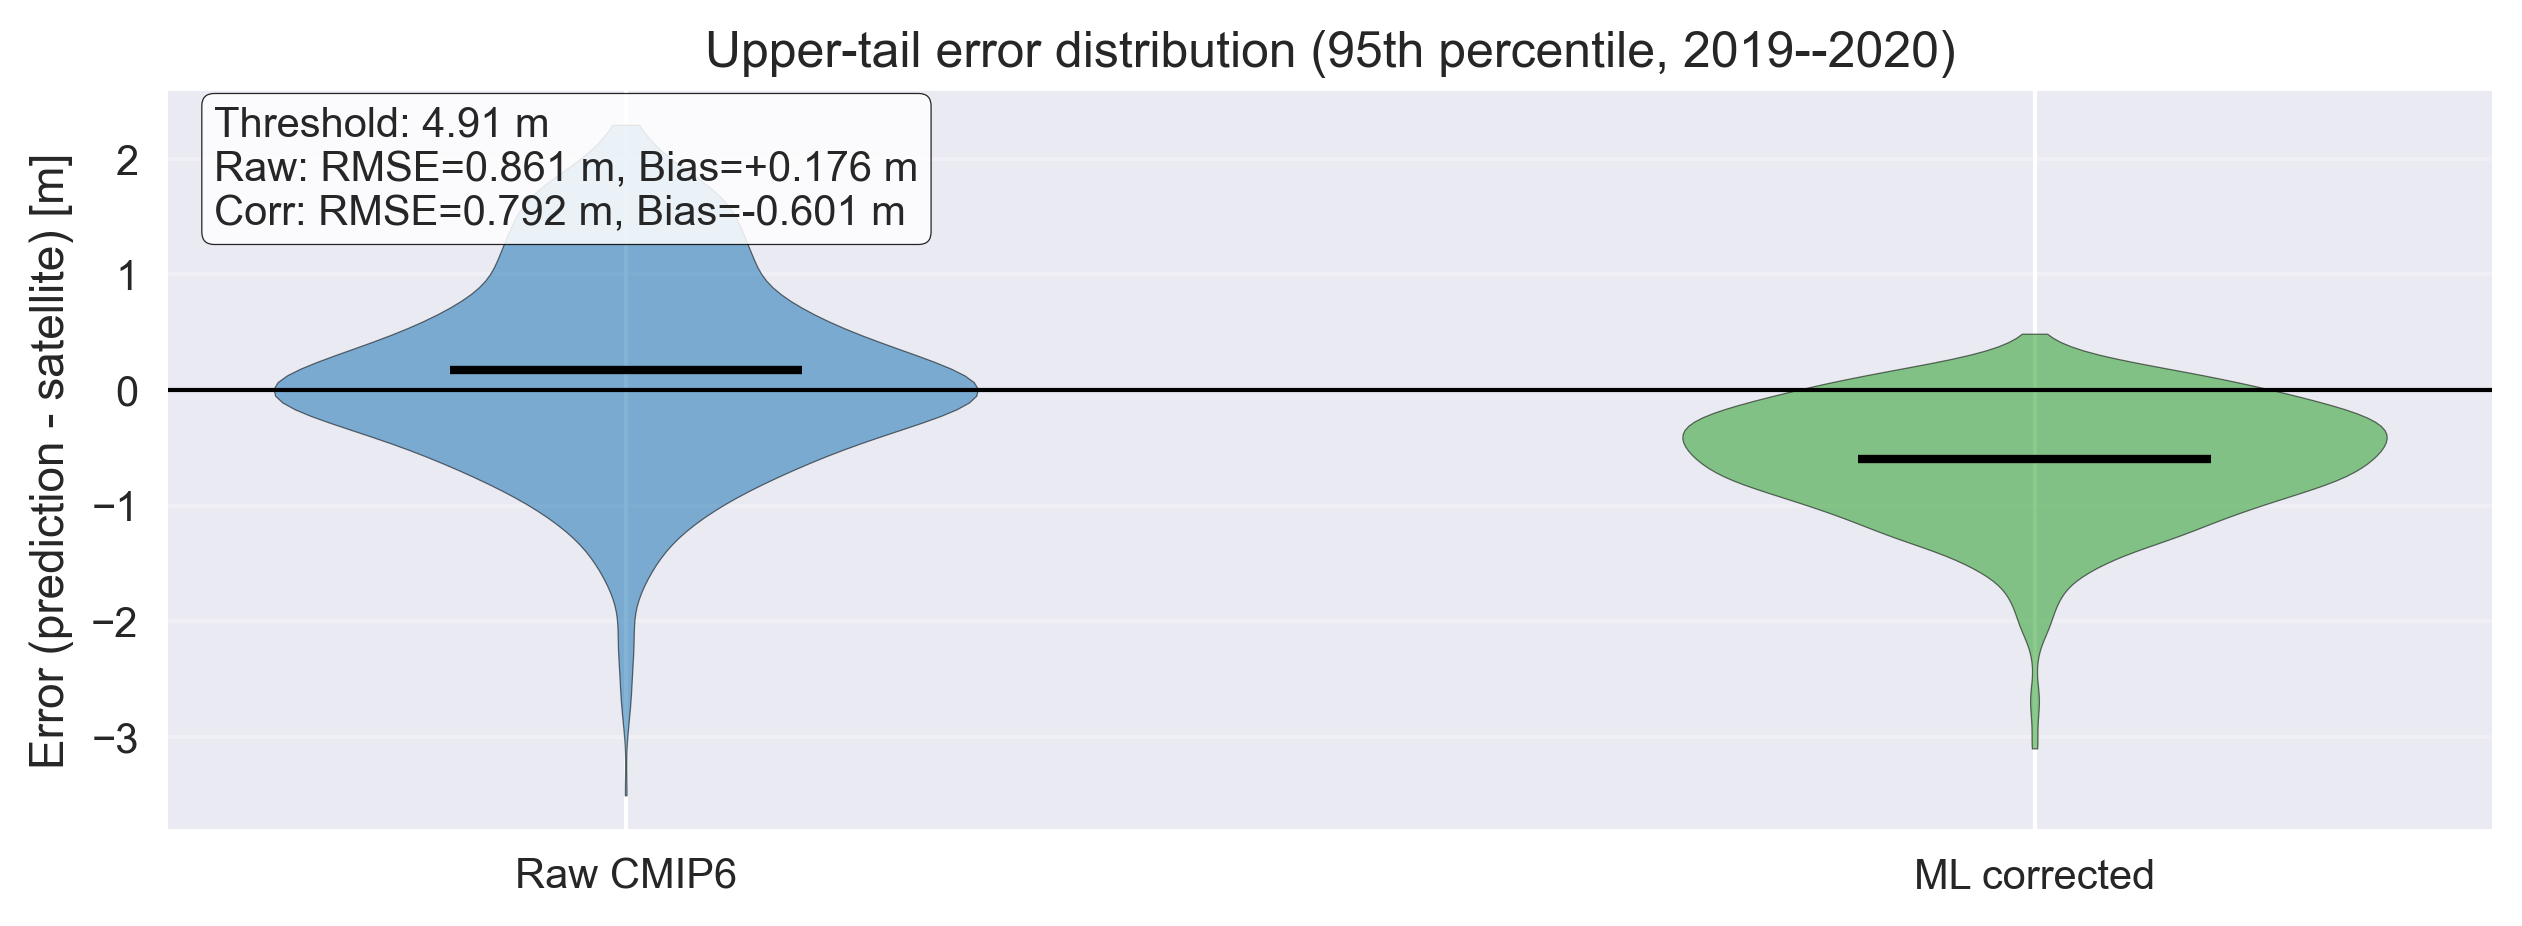
\includegraphics[width=0.8\linewidth,height=0.65\textheight,keepaspectratio]{plots/tail_performance.png}
  \vspace{0.2cm}
  
  \small{The model performs well even for extreme events (top 5\% of wave heights), reducing the underestimation often seen in climate models during storm conditions.}
\end{frame}

\begin{frame}{Benchmarks: Computational Cost}
  \setfooter{Computational efficiency comparison across different ML architectures}
  \centering
  \textbf{Computational Cost}
  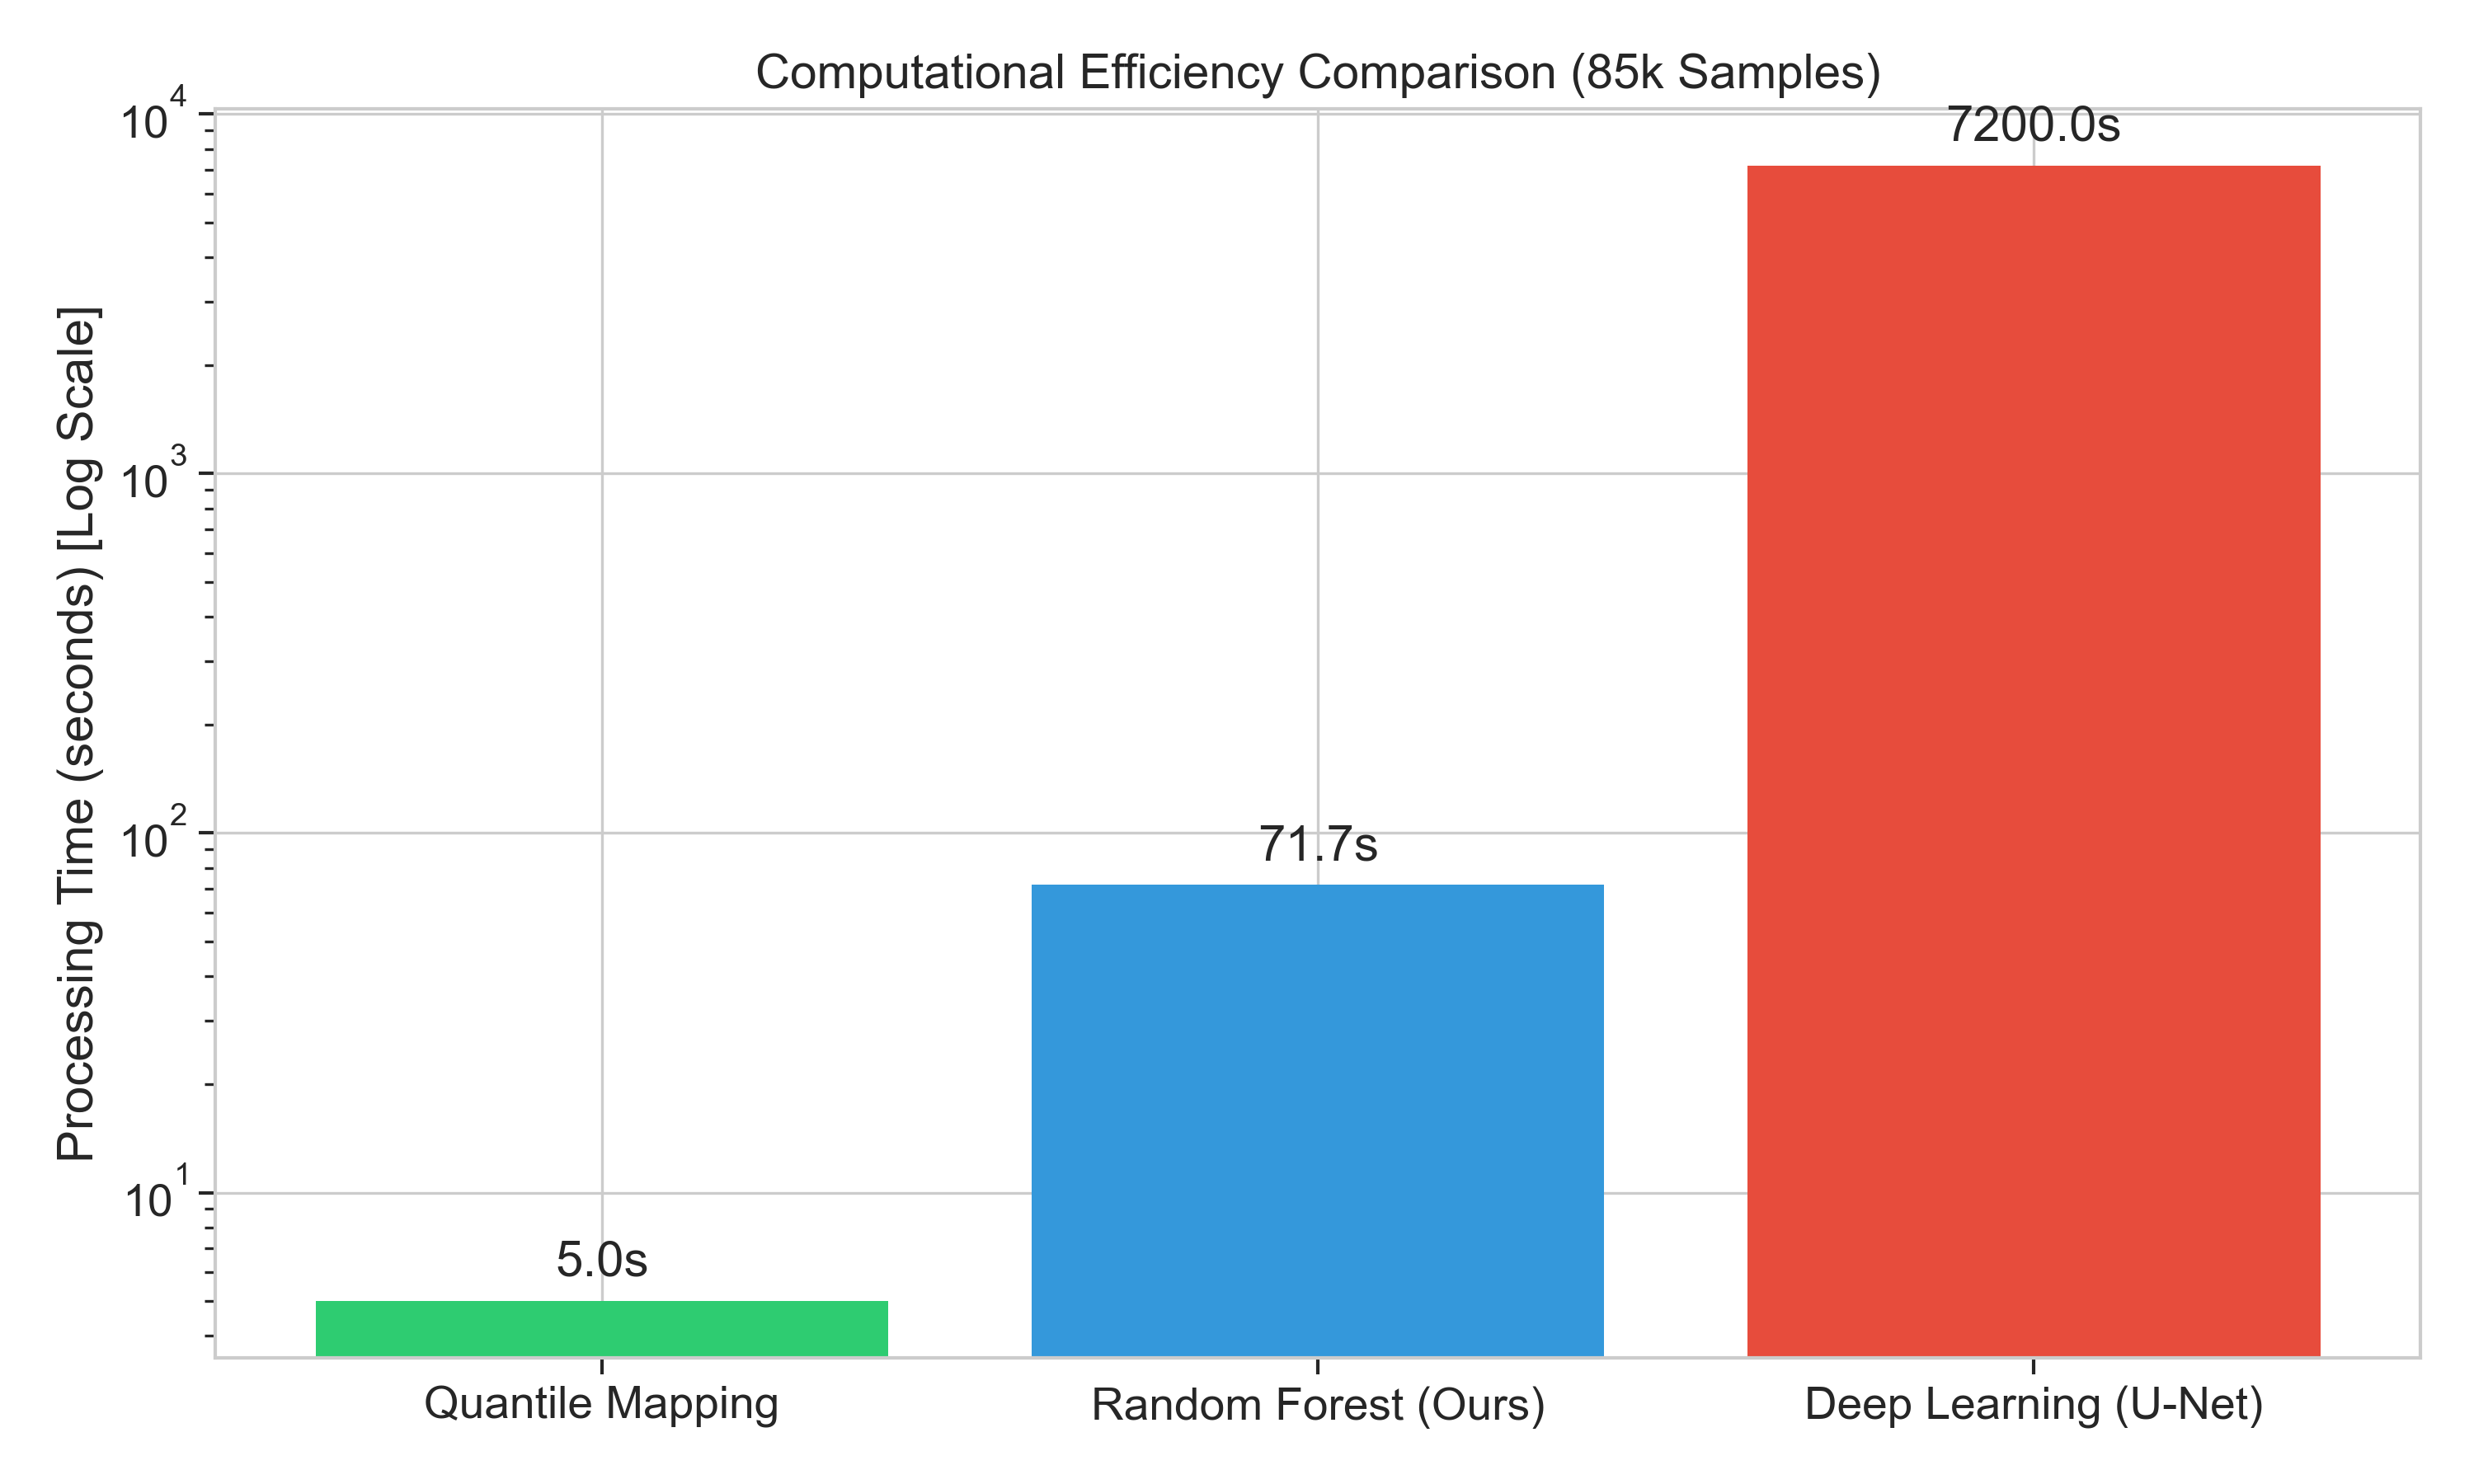
\includegraphics[width=0.8\linewidth,height=0.65\textheight,keepaspectratio]{plots/computational_benchmark.png}
  \vspace{0.2cm}
  
  \small{Our Random Forest approach offers a balanced trade-off, providing high accuracy with significantly lower computational cost compared to deep learning methods like CNNs or LSTMs.}
\end{frame}

\begin{frame}{Results (Initial Summary)}
  \setfooter{Overview of error reduction for both SWH and SLA variables}
  \begin{columns}[T,onlytextwidth]
    \begin{column}{0.52\textwidth}
      \begin{block}{Test Performance (Unseen Data)}
        \centering
        \scriptsize
        \setlength{\tabcolsep}{3pt}
        \renewcommand{\arraystretch}{1.12}
        \resizebox{\linewidth}{!}{%
          \begin{tabular}{@{}lccc@{}}
            \toprule
            Variable & Error Before & Error After & Improvement \\ \midrule
            SWH (Indian Ocean) & 0.599\,m & 0.308\,m & $\sim$48\% \\
            SLA (initial test) & 0.1037\,m & 0.0578\,m & 44.3\% \\
            \bottomrule
          \end{tabular}%
        }
      \end{block}
      \begin{block}{Key takeaways}
        \begin{itemize}
          \item SWH correction is robust over the Indian Ocean.
          \item SLA work is preliminary (specific timeline only) and needs extension to longer periods.
          \item Errors follow specific patterns in space and time; our tool captures this well.
        \end{itemize}
      \end{block}
    \end{column}
    \begin{column}{0.48\textwidth}
      \centering
      % Plot 1: SWH Error Reduction
      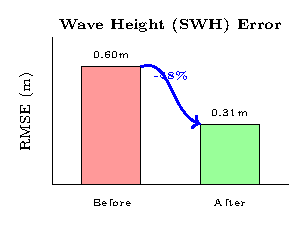
\includegraphics[width=0.7\linewidth,height=0.30\textheight,keepaspectratio]{swh_chart.pdf}
      
      \vspace{0.1cm}
      
      % Plot 2: SLA Error Reduction
      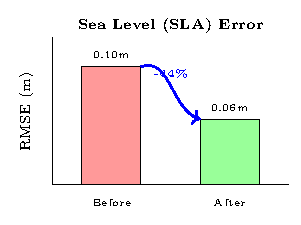
\includegraphics[width=0.7\linewidth,height=0.30\textheight,keepaspectratio]{sla_chart.pdf}
    \end{column}
  \end{columns}
\end{frame}

\section{Work Proposed During the Next Year}
\begin{frame}{Work Proposed During the Next Year}
  \setfooter{Future milestones: Extending dataset and uncertainty analysis}
  \begin{itemize}
    \item Apply this method to the full 8-year dataset (2015--2023) for the Indian Ocean.
    \item Test it on more sub-regions and different climate models.
    \item Estimate our confidence levels for every prediction (uncertainty analysis).
    \item Use the proven tool to correct future climate forecasts (SSP scenarios) and share the data.
  \end{itemize}
\end{frame}

\section{Conclusion}
\begin{frame}{Conclusion}
  \setfooter{Project summary and key takeaways from initial research}
  \begin{itemize}
    \item Created a complete system to check and fix climate model errors using satellites.
    \item Early tests show we cut the errors by nearly half (significant improvement).
    \item Coming up: Applying this to future climate scenarios to help decision-making.
  \end{itemize}
\end{frame}

\section{References}
\begin{frame}[allowframebreaks]{References}
  \setfooter{Relevant literature and project citations}
  \scriptsize
  \begin{thebibliography}{10}

    \bibitem{lemos2020}
    G. Lemos, M. Menendez, A. Semedo, J. P. Reis, and T. A. Adcock, ``On the need of bias correction methods for wave climate projections,'' \textit{Global Planet. Change}, vol. 186, p. 103114, 2020.

    \bibitem{sun2022}
    D. Sun, W. Huang, Y. Luo, J. S. Wright, H. Fu, and B. Wang, ``A deep learning-based bias correction method for predicting ocean surface waves in the Northwest Pacific Ocean,'' \textit{Geophys. Res. Lett.}, vol. 49, no. 23, e2022GL100916, 2022.

    \bibitem{campos2018}
    R. M. Campos, C. Guedes Soares, and L. Alves, ``Extreme wave climate variability in the North Atlantic Ocean,'' \textit{Ocean Eng.}, vol. 150, pp. 199--210, 2018.

    \bibitem{cannon2018}
    A. J. Cannon, ``Multivariate quantile mapping bias correction: an N-dimensional probability density function transform for climate model simulations,'' \textit{Clim. Dyn.}, vol. 50, no. 1, pp. 31--49, 2018.

    \bibitem{reichstein2019}
    M. Reichstein \textit{et al.}, ``Deep learning and process understanding for data-driven Earth system science,'' \textit{Nature}, vol. 566, no. 7743, pp. 195--204, 2019.

    \bibitem{breiman2001}
    L. Breiman, ``Random forests,'' \textit{Mach. Learn.}, vol. 45, no. 1, pp. 5--32, 2001.

    \bibitem{ellenson2020}
    A. Ellenson, C. Pei, L. \"Ozkan-Haller, F. Fiedler, and T. Haller, ``An application of a machine learning algorithm to determine and describe error patterns in wave model datasets,'' \textit{Coastal Eng.}, vol. 157, p. 103595, 2020.

    \bibitem{lemos2020b}
    G. Lemos, A. Semedo, M. Dobrynin, M. Menendez, and P. M. Miranda, ``Bias-corrected CMIP5-derived single-forcing future wind-wave climate projections,'' \textit{J. Appl. Meteorol. Climatol.}, vol. 59, no. 9, pp. 1525--1547, 2020.

    \bibitem{patra2023}
    A. Patra \textit{et al.}, ``Historical global ocean wave data simulated with CMIP6 anthropogenic and natural forcings,'' \textit{Sci. Data}, 2023.

    \bibitem{meucci2024}
    A. Meucci \textit{et al.}, ``An 8-model ensemble of CMIP6-derived ocean surface wave climate,'' \textit{Sci. Data}, 2024.

  \end{thebibliography}
\end{frame}

\end{document}
